\label{sec:hadhad_multijet}

\todo[inline]{Maybe say that we perform some tricks to go from
  ``event-level'' fake factors to ``tau-level'' fake factors?}

Multi-jet production is a source of background in the \hadhad signal
region where both \tauhadvis candidates originate from the
misidentification of quark- or gluon-initiated jets. It represents the
second largest background with \faketauhadvis in the \hadhad SR after
the dominant \ttbarFakes contribution.

\subsubsection{The fake factor method}

The multi-jet background is estimated using the fake factor method
which is a data-driven method for background estimation. It is
applicable in cases where two event observables exist that are
statistically independent for the background process to be estimated,
while also being strong discriminators between the background and
other processes (signal and non-multi-jet processes). Four disjoint
regions can be defined, three background-enriched control regions and
a signal-like region, by performing a binary categorisation of each
observable. The assumption of statistical independence allows to
relate the expected number of events for the background process
between the control regions and the signal-like region, thus yielding
a data-driven estimate of the expected background contribution in the
signal-like region.

In the \hadhad channel, two observables that allow to define control
regions enriched in multi-jet events are the \tauid requirements
fulfilled by the \tauhadvis candidates and the sign of the electric
charges of both candidates.

In the signal region, \tauhadvis candidates are required to pass the
loose \tauid working point. This requirement defines regions where
both \tauhadvis candidates pass identification, herafter referred to
as ID regions. The selection is partially inverted to obtain control
regions enhanced in multi-jet events by requiring that exactly one
\tauhadvis candidate is failing the loose \tauid working point while
still passing a working point corresponding to an efficiency loss of
\tauhad of about 1\,\% ($\text{RNN score} > 0.01$). The \tauhadvis
candidates fulfilling this selection are referred to as
anti-\tauhadvis and the regions defined by the inversion of the
identification criterion as Anti-ID regions. The identification
criterion cannot be fully inverted due to a pre-selection applied in
the data reduction pipeline of the ATLAS experiment\footnote{In the
  ATLAS collaboration, datasets targeting $\PHiggs \to \hadhad$
  processes require events with at least one \tauhadvis passing the
  loose \tauid working point and one \tauhadvis with a \tauid score
  exceeding 0.01.}. However, the fake factor method is still valid in
the presence of these constraints provided the underlying assumptions
of the method hold.

The electric charge of both \tauhadvis candidates produced from signal
processes and dominant sources of backgrounds with two \tauhadvis
orginating for hadronic $\tau$~decays ($\PZ \to \tautau$,
$\PHiggs \to \tautau$, \ttbar) are expected to be reconstructed with
opposite-sign (OS) electric charge. The OS requirement is inverted
yielding regions with \tauhadvis candidates of same-sign (SS) electric
charge, depleting the region of processes where both \tauhadvis
orginate from hadronic $\tau$ decays. In contrast, the multi-jet
background contributes similarly to the OS and SS regions since
\tauhadvis charge reconstruction has little sensitivity to the
relative sign of the electric charge between partons initiating jets
that are being misidentified as \tauhadvis.

With the previously defined control regions and the assumption of
independence of the observables defining the regions, the expected
multi-jet contribution in regions with \tauhadvis passing loose
identification and with \tauhadvis pairs of opposite-sign electric
charge can be estimated using
\begin{align*}
  N_\text{multi-jet}^{\text{OS, ID}} =
  N_\text{multi-jet}^{\text{OS, Anti-ID}}
  \cdot
  \underbrace{\frac{N_\text{multi-jet}^{\text{SS, ID}}}
  {N_\text{multi-jet}^{\text{SS, Anti-ID}}}}
  _{= \text{FF}_\text{SS}} \,\text{,}
\end{align*}
where $N_\text{multi-jet}$ is the number of multi-jet events in a
given region. The fake factor (FF) measures the ratio of multi-jet
events in the ID and Anti-ID region\footnote{The use of identification
  or isolation criteria to defining the ratio is the main difference
  between the fake factor method and the more general ABCD method.}.

The control regions defined by inverting the OS and/or ID requirements on
\tauhadvis do not provide pure samples of multi-jet events. Therefore,
number of multi-jet events is estimated according to
\begin{align*}
  N_\text{multi-jet} = N_\text{data} - N_\text{non-multi-jet} \,\text{,}
\end{align*}
where $N_\text{data}$ is the observed number of events in the
multi-jet enriched region and $N_\text{non-multi-jet}$ the expected
contribution of non-multi-jet events estimated using simulation.

The probability of misidentifying a quark- or gluon-jet as a hadronic
$\tau$ decay depends on the properties of the reconstructed \tauhadvis
candidate. Particularly, the reconstructed decay mode and visible
transverse momentum affect the probability of a jet reconstructed as a
\tauhadvis to pass \tauid (cf.\ \Cref{sec:tauid}). To control for this
effect, the fake factor method is commonly performed in bins of
observables related to the properties of reconstructed \tauhadvis.

In~\Cref{tab:mjfakes_yields} the multi-jet and non-multi-jet yields in
the regions relevant for the \faketauhadvis estimation are
summarised. The 2 $b$-tag region, while most similar to the signal
region, is not well suited to estimate fake factors:
\begin{itemize}

\item The 2 $b$-tag regions used for the measurement of fake factors
  have a large contamination from non-multi-jet backgrounds, primarily
  \ttbarFakes, that have to be subtracted. The large size of the
  subtraction leads to a degradation of the statistical precision of
  measured fake factors and inflates systematic uncertainties
  originating from the modelling of the subtracted components.

\item The strict \btag requirement suppresses the multi-jet
  contribution in the control regions preventing a differential
  measurement of fake factors in properties of the \tauhadvis.

\item The multi-jet estimate cannot be validated in the 2 $b$-tag
  region due to the absence of a region with high multi-jet purity
  that is similar to the signal region.

  % Resultingly, the statistical independence of the charge sign and ID
  % observables employed by the FF method cannot be verified.
\end{itemize}
These issues are addressed by performing the fake factor measurement
in the 1 $b$-tag region instead, which has a higher abundance and
purity of multi-jet events, and extrapolating the measurement into the
2 $b$-tag region to obtain a multi-jet background estimate in the
signal region. Distributions of the \pT of the leading and sub-leading
\tauhadvis candidates in the regions relevant to the fake factor
measurement are shown in~\Cref{fig:mjfakes_1tag_ss_plots}.

\begin{table}[htbp]
  \centering

  \begin{subtable}[t]{\textwidth}
    \centering
    % Size of subtraction and multi-jet purity:
%                         multi_jet  non_multi_jet  multi_jet_error  non_multi_jet_error  multi_jet_purity
% anti_id charge_sign
% False   OS           16067.048497   16443.951503       204.558258            96.607872          0.494203
%         SS           14040.394005    1971.605995       129.147367            25.827164          0.876867
% True    OS           91582.182374   13677.817626       334.090987            79.729466          0.870057
%         SS           78399.983641    5707.016359       296.470480            61.544664          0.932146

\begin{tabular}{
  ll
  S[table-format=5.0(3)]
  S[table-format=5.0(3)]
  c}
  \toprule
  \multicolumn{2}{l}{Region} & {$N_\text{multi-jet}$} & {$N_\text{non-multi-jet}$} & {Multi-jet purity} \\
  \midrule
  \multirow{2}{*}{SS} & ID      & 14040 +- 130 & 1970 +- 30   & 88\,\% \\
                      & Anti-ID & 78400 +- 300 & 5710 +- 70   & 93\,\% \\
  \midrule
  \multirow{2}{*}{OS} & ID      & 16070 +- 210 & 16440 +- 100 & 49\,\% \\
                      & Anti-ID & 91580 +- 340 & 13680 +- 80  & 87\,\% \\
  \bottomrule
\end{tabular}



%%% Local Variables:
%%% mode: latex
%%% TeX-master: "../phd_thesis"
%%% End:

    \subcaption{1 $b$-tag regions}
    \label{tab:mjfakes_yields_1tag}
  \end{subtable}

  \begin{subtable}[t]{\textwidth}
    \centering
    % Size of subtraction and multi-jet purity:
%                        multi_jet  non_multi_jet  multi_jet_error  non_multi_jet_error  multi_jet_purity
% anti_id charge_sign
% False   OS            408.197943    7971.802057       105.950917            53.344135          0.048711
%         SS           1299.622259    1001.377741        50.345854            15.287412          0.564808
% True    OS           8429.603396    8864.396604       139.699303            47.136984          0.487429
%         SS           7653.735896    3338.264104       108.557939            28.157166          0.696301

\begin{tabular}{
  ll
  S[table-format=5.0(3)]
  S[table-format=5.0(3)]
  c}
  \toprule
  \multicolumn{2}{l}{Region} & {$N_\text{multi-jet}$} & {$N_\text{non-multi-jet}$} & {Multi-jet purity} \\
  \midrule
  \multirow{2}{*}{SS} & ID      & 1300 +- 60  & 1000 +- 20 & 56\,\% \\
                             & Anti-ID & 7650 +- 110 & 3340 +- 30 & 70\,\% \\
  \midrule
  \multirow{2}{*}{OS} & ID      & \multicolumn{3}{c}{\rule[3pt]{5.2em}{0.3pt}\hspace{1em}Signal Region\hspace{1em}\rule[3pt]{5.2em}{0.3pt}} \\
                             & Anti-ID & 8430 +- 140 & 8860 +- 50 & 49\,\% \\
  \bottomrule
\end{tabular}




%%% Local Variables:
%%% mode: latex
%%% TeX-master: "../phd_thesis"
%%% End:

    \subcaption{2 $b$-tag regions}
  \end{subtable}

  \caption{Number of multi-jet events in regions defined by the
    electric charge of the \tauhadvis pair (OS, SS) and \tauhadvis
    identification (ID, Anti-ID). The number of multi-jet events,
    $N_\text{multi-jet}$, is estimated by subtracting the number
    non-multi-jet events, $N_\text{non-multi-jet}$, estimated using
    simulation from the observed number of events in this region. The
    breakdown is shown after the 1 $b$-tag requirement in (a); after
    the 2 $b$-tag requirement in (b). The signal region (2 $b$-tag OS
    ID) is omitted. Uncertainties are from data and MC statistical
    sources only.}
  \label{tab:mjfakes_yields}
\end{table}

\begin{figure}[htbp]
  \centering

  \begin{subfigure}{0.49\textwidth}
    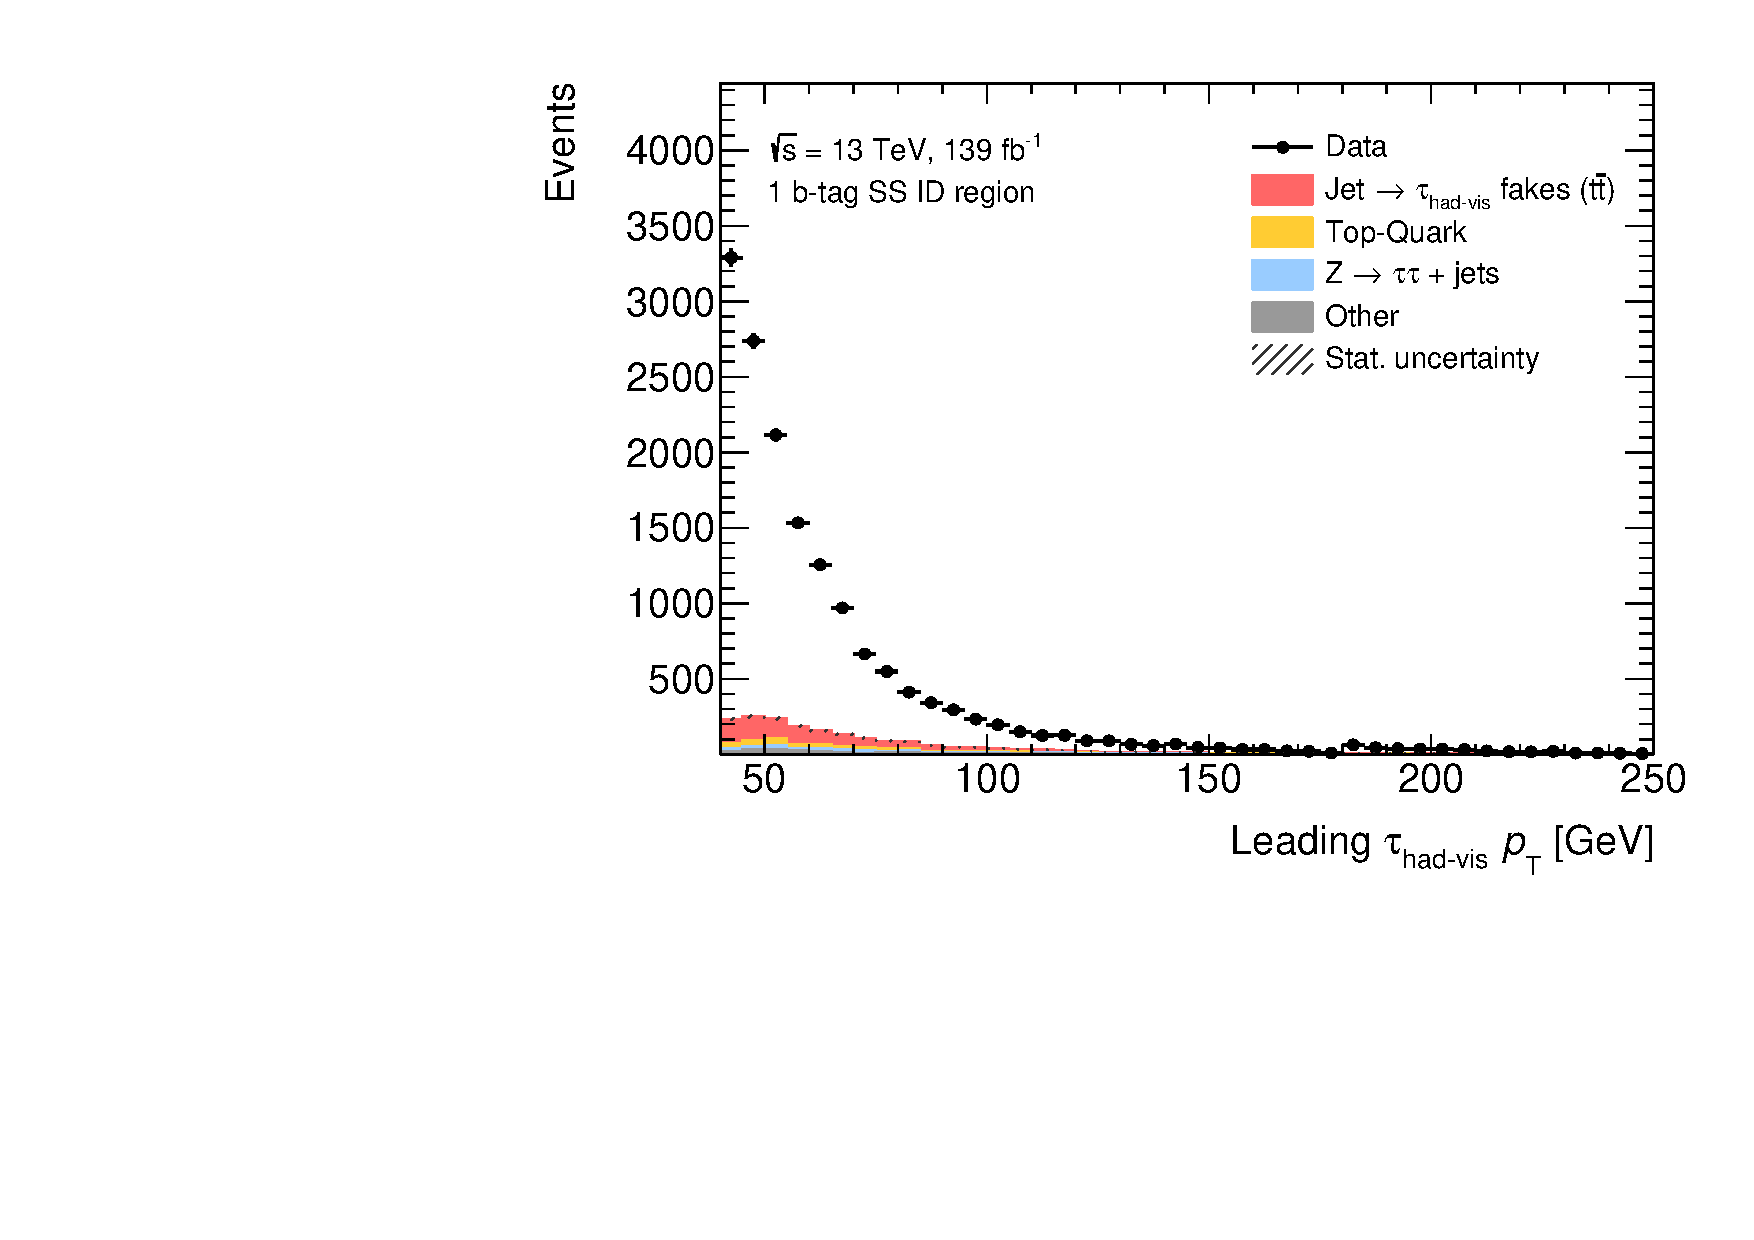
\includegraphics[width=\textwidth]{fakefactors/region_plots/tau0pt_1tag_ss_id}
    \subcaption{1 $b$-tag SS ID region}
  \end{subfigure}
  \begin{subfigure}{0.49\textwidth}
    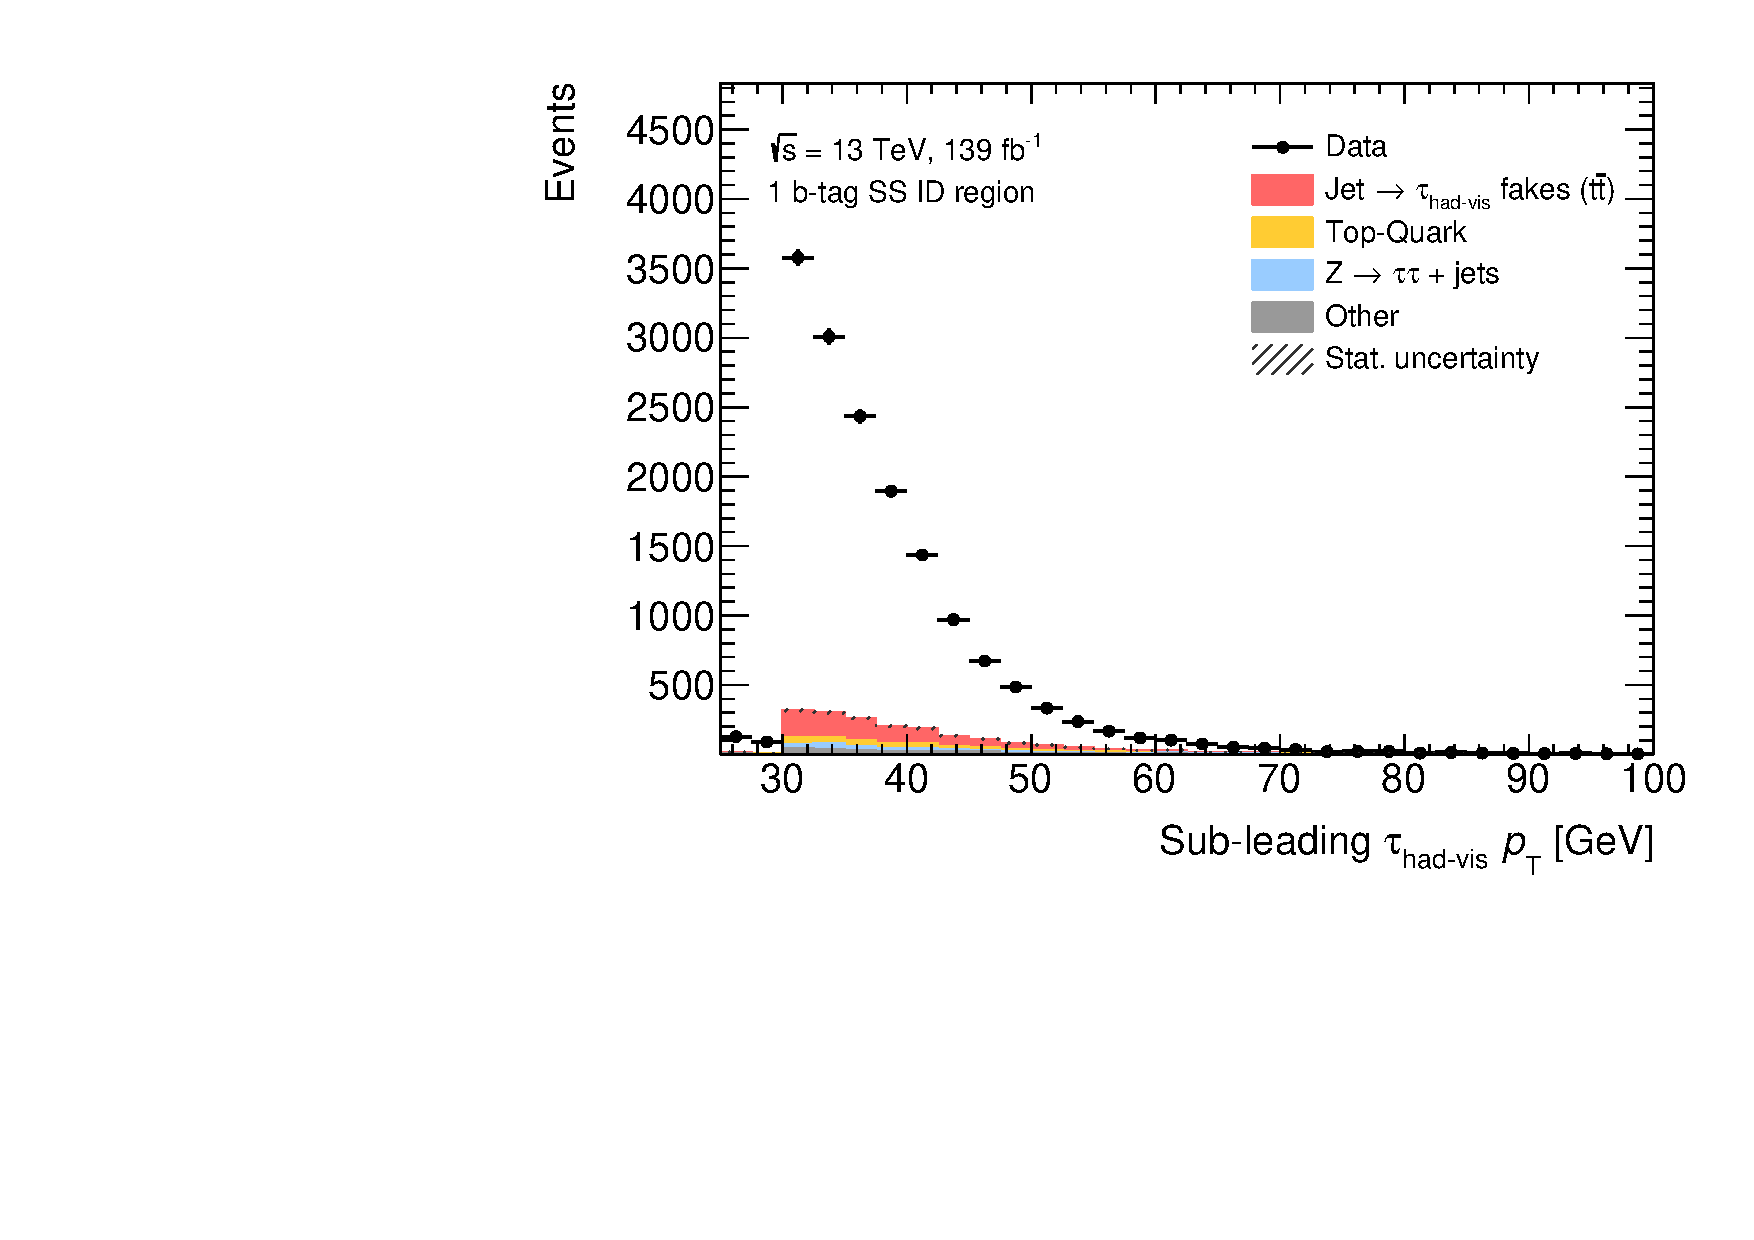
\includegraphics[width=\textwidth]{fakefactors/region_plots/tau1pt_1tag_ss_id}
    \subcaption{1 $b$-tag SS ID region}
  \end{subfigure}

  \begin{subfigure}{0.49\textwidth}
    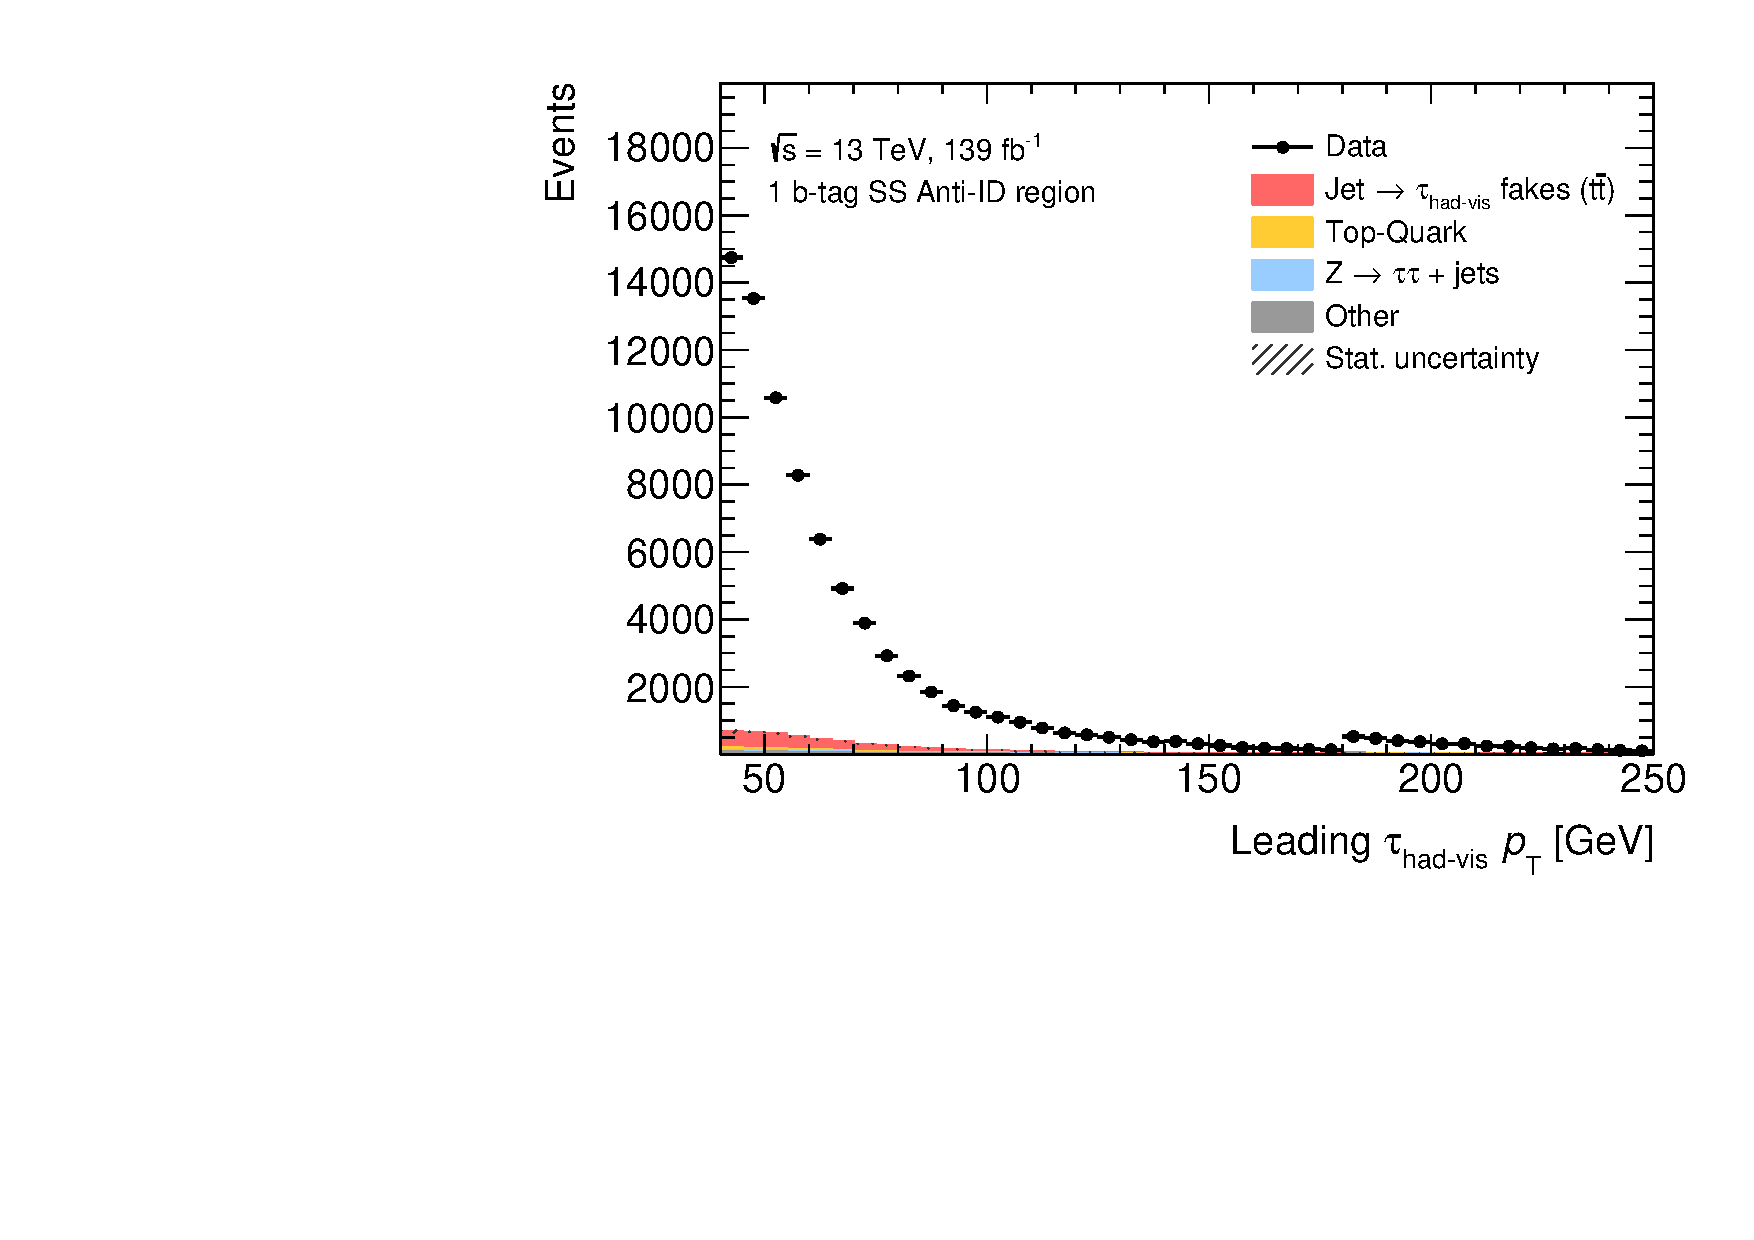
\includegraphics[width=\textwidth]{fakefactors/region_plots/tau0pt_1tag_ss_antiid}
    \subcaption{1 $b$-tag SS Anti-ID region}
  \end{subfigure}
  \begin{subfigure}{0.49\textwidth}
    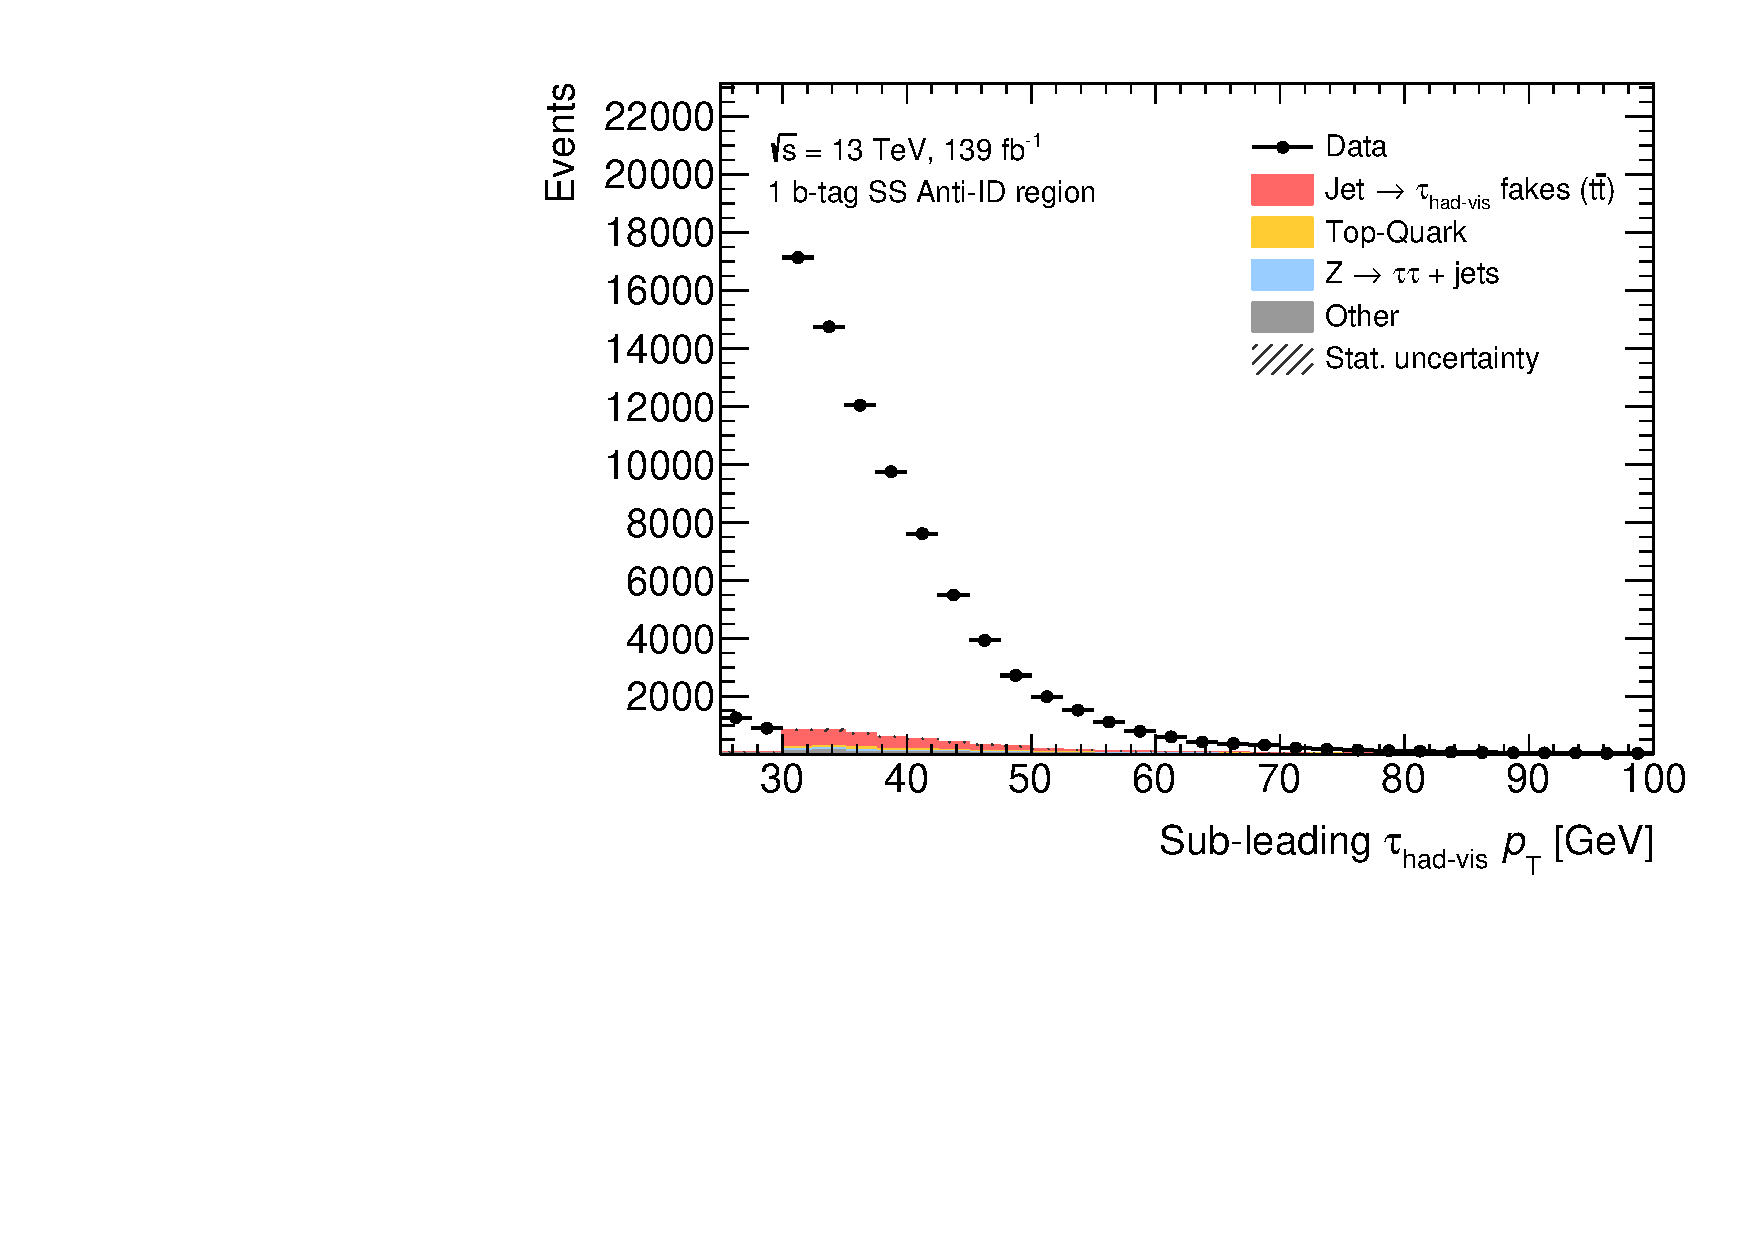
\includegraphics[width=\textwidth]{fakefactors/region_plots/tau1pt_1tag_ss_antiid}
    \subcaption{1 $b$-tag SS Anti-ID region}
  \end{subfigure}

  \caption{Distribution of leading and sub-leading \tauhadvis \pT for
    observed data and non-multi-jet backgrounds in regions entering
    the fake factor measurement. The 1 $b$-tag SS ID region is shown
    in (a,b) and the 1 $b$-tag SS Anti-ID region in (c,d). Coloured
    histograms depict the contributions of non-multi-jet processes
    that are subtracted during the fake factor measurement. The
    difference between the observed data and the non-multi-jet
    background estimate is attributed to the missing multi-jet
    background estimate. All regions are shown at pre-selection level
    corresponding to the SS region yields and multi-jet purities
    listed in~\Cref{tab:mjfakes_yields_1tag}.}%
  \label{fig:mjfakes_1tag_ss_plots}
\end{figure}

A schematic illustration of the approach is givens
in~\Cref{fig:fakefactor_regions}. Fake factors measured in the 1
$b$-tag regions ($\text{FF}_\text{SS}^\text{1-tag}$) are applied to
events in the 2 $b$-tag OS Anti-ID region after subtraction of
non-multi-jet contributions to obtain an estimate of the multi-jet
background in the signal region. Multiplicative transfer factors
($\text{TF}_{1 \ra 2\,b\text{-tag}}$) are applied to
$\text{FF}_\text{SS}^\text{1-tag}$ when used in 2 $b$-tag regions,
absorbing possible differences between fake factors measured in 1 and
2 $b$-tag regions and the uncertainties associated with this
extrapolation.

\begin{figure}[htbp]
  \centering

  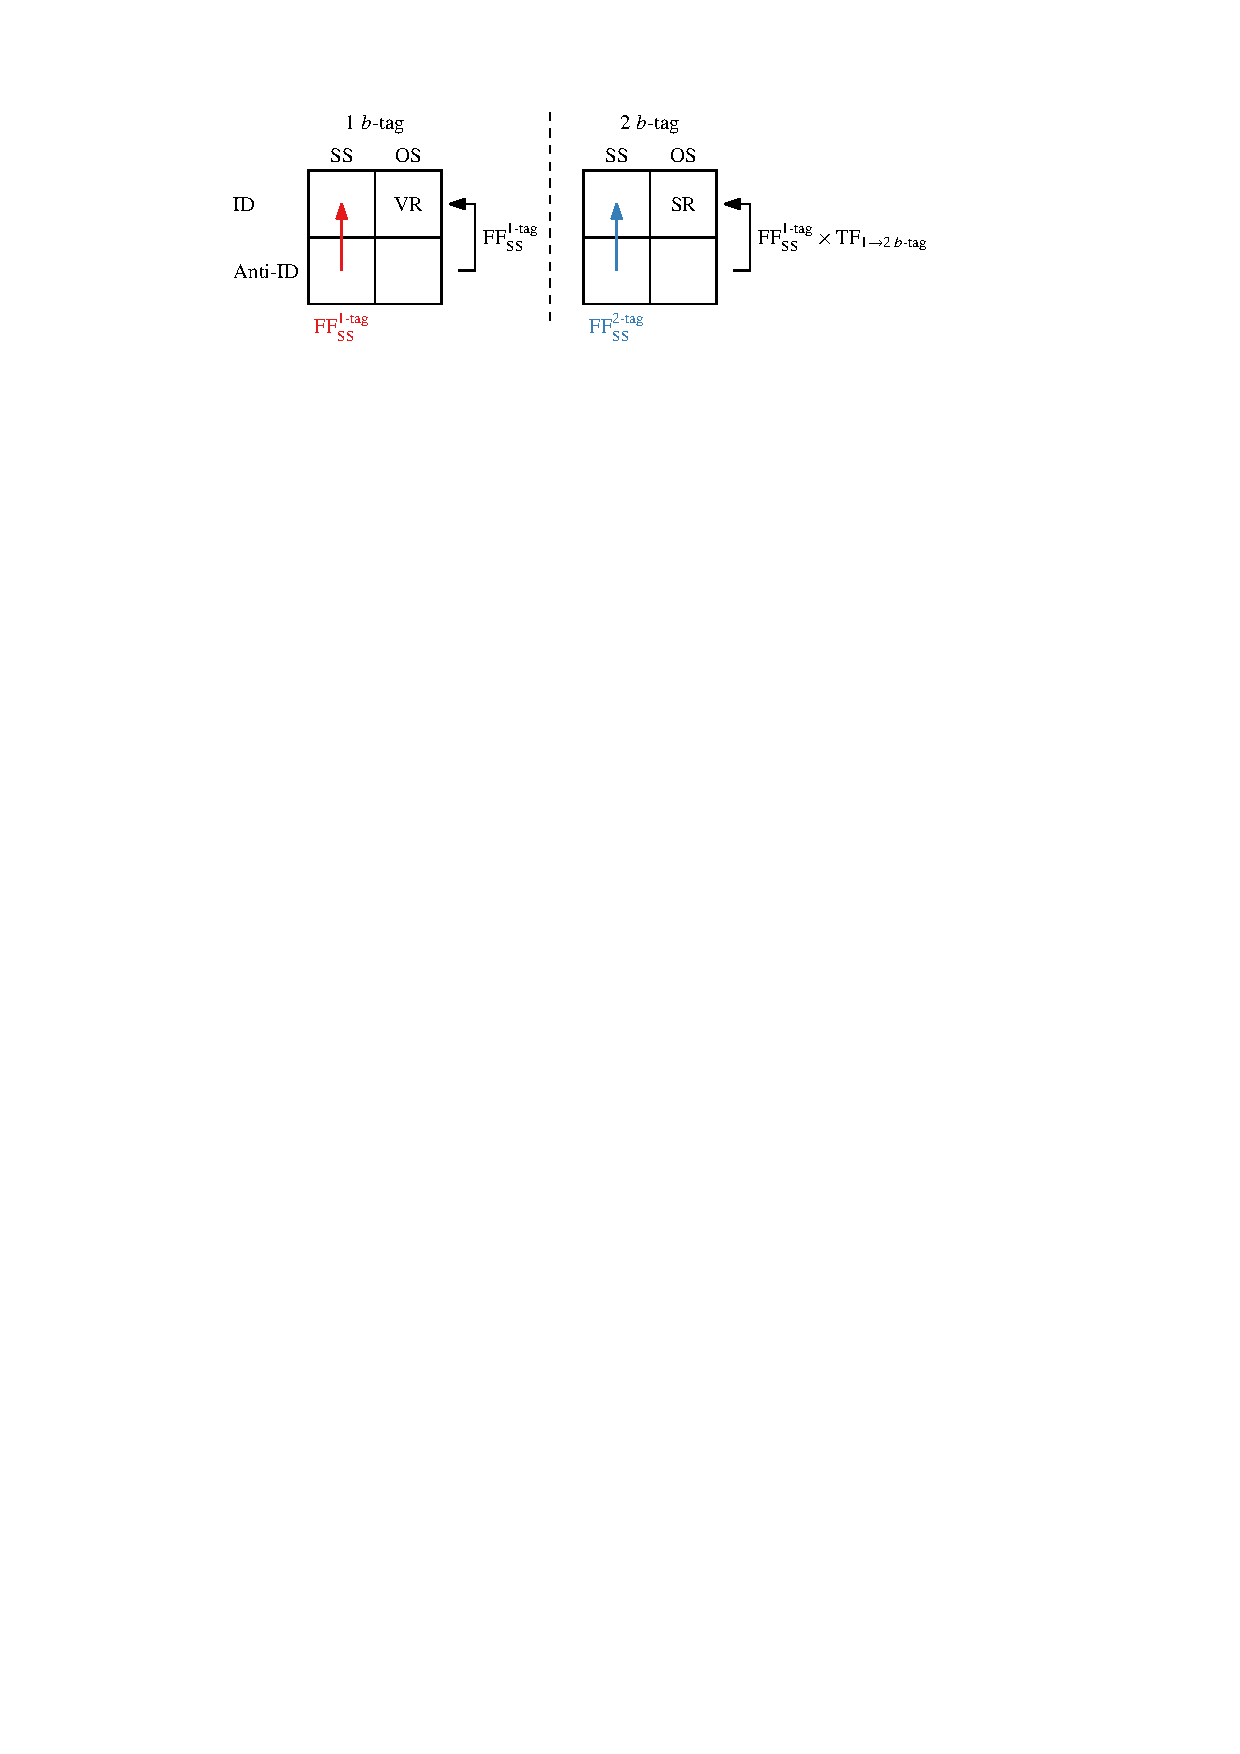
\includegraphics[scale=1]{fakefactors/regions}

  \caption{Schematic description of the fake factor method employed to
    estimate the multi-jet background in the signal region of the
    \hadhad channel. The squares represent the multi-jet events
    ($N_\text{multi-jet} = N_\text{data} - N_\text{non-multi-jet}$) in
    a particular region. The coloured arrows correspond to fake
    factors calculated as the ratio of multi-jet events in ID and
    Anti-ID regions.}
  \label{fig:fakefactor_regions}
\end{figure}

The 1 $b$-tag OS ID region serves as a validation region to check the
agreement of the total background prediction with the observed
data. Any non-closure observed in this region indicates either a
violation of the assumptions of the fake factor method, or a
parametrisation of the fake factors that is insufficient for the
modelling of the multi-jet background.

% % verify the independence of the observables related to \tauid and
% % electric charge of the \tauhadvis pair.
% This approach is equivalent to a comparison of fake factors measured
% in the OS and SS regions\footnote{\Cref{tab:mjfakes_yields_1tag} can
%   be used to calculate inclusive fake factors in the OS and SS
%   regions, yielding
%   $\text{FF}_\text{SS}^\text{1-tag} \approx
%   \text{FF}_\text{OS}^\text{1-tag} \approx 0.18$, which is a
%   sufficient condition for statistical independence of the fake factor
%   observables at the level of the inclusive selection.}, which have to
% agree under the assumptions of the method.\todo{Needs some work...}


\subsubsection{Measurement of fake factors}

% Binning in years / trigger
The fake factor measurement is performed separately for events
selected by single- and di-\tauhadvis triggers as well as the years of
data collection. During Run~2 of the LHC different \tauhadvis trigger
chains were used by the ATLAS experiment to collect the data used in
this analysis. As a result, the topologies of selected events and the
\tauid applied at the high-level trigger changed as Run~2
progressed. To account for possible differences resulting from the
change in trigger-selection, the fake factor measurement is performed
separately for three major data collection periods: 2015-2016, 2017,
and 2018.
% The 1 $b$-tag SS regions relevant to the measurement of fake factors
% are shown in~\Cref{fig:mjfakes_1tag_ss_plots}.

% Reason for binning in
The categorisation of the fake factors by trigger that selected the
event is further motivated by the differences between single- and
di-\tauhadvis triggers. Single-\tauhadvis triggers require one
\tauhadvis candidate with high transverse momentum that is identified
at the HLT without any selections applied to the other candidate. In
contrast, di-\tauhadvis triggers require two \tauhadvis to be
identified at the HLT with similar transverse momentum thresholds
applied to both. This allows \tauhadvis candidates in in the
di-\tauhadvis trigger category to be treated equally once
\pT-threshold effects are accounted for. This is not the case for
events selected by single-\tauhadvis triggers.

Dependencies of the fake factors on reconstructed quantities of
\tauhadvis candidates are accounted for by further categorisation
based on properties of the (anti-)\tauhadvis that distinguishes the ID
from the Anti-ID regions. The fake factor measurement is performed
separately for 1- and 3-prong \tauhadvis candidates for both trigger
categories.

Fake factors for events selected by di-\tauhadvis triggers are
additionally measured in bins of \tauhadvis~\pT and separately for
\tauhadvis in the barrel and endcap regions of the ATLAS detector.

In contrast, few multi-jet events enter the single-\tauhadvis trigger
category due to large \pT thresholds on the leading \tauhadvis. This
prevents a further subdivision of the fake factor measurement in this
category into many bins. Therefore, the fake factors for
singe-\tauhadvis trigger events are measured separately for cases
where the anti-\tauhadvis is leading and the sub-leading in \pT. This
accounts for differences in HLT \tauid and the typically large
differences in \pT between the leading and sub-leading
\tauhadvis~candidates.

\subsubsection{Measurement of fake factors: di-\tauhadvis triggers}

{% Group for extra definitions
  \newcommand*{\ffargs}{\ensuremath{( \myvec{x}_{\tau} )}\xspace}

  \newcommand*{\NmjID}[2]{\ensuremath{N_\text{multi-jet}^{\text{#1, loose }\tau_{#2}}}\xspace}
  \newcommand*{\NmjIDIncl}[1]{\ensuremath{N_\text{multi-jet}^{\text{#1, ID}}}\xspace}

  \newcommand*{\NmjAntiIDIncl}[1]{\ensuremath{N_\text{multi-jet}^{\text{#1, Anti-ID}}}\xspace}
  \newcommand*{\NmjAntiID}[2]{\ensuremath{N_\text{multi-jet}^{\text{#1, anti-}\tau_{#2}}}\xspace}

  The Anti-ID region can be partitioned into two sub-regions: one
  where the anti-\tauhadvis is the leading and one where it is the
  sub-leading \tauhadvis candidate. Provided the conditions for the
  fake factor method are fulfilled, both regions can be used to obtain
  separate estimates of the multi-jet background in the OS ID
  region. The notation used to describe the fake factor measurement is
  introduced in the following:
  \begin{description}[style=standard]
  \item[$\tau_0$ ($\tau_1$)] The \tauhadvis candidate leading (sub-leading) in \pT.

  \item[$\myvec{x}_\tau$] A vector of categorical observables related
    to a \tauhadvis that defines the bin of the fake factor
    measurement. The measurement in the di-\tauhadvis trigger category
    is performed separately for 1- and 3-prong \tauhadvis, and in bins
    of \tauhadvis \pT and $\eta$.

  \item[$\NmjID{SS(OS)}{i}\ffargs$] The estimated number of multi-jet
    events in the SS (OS) ID region where~$\tau_i$ has
    observables~$\myvec{x}_\tau$.

  \item[$\NmjAntiID{SS(OS)}{i}\ffargs$] The estimated number of
    multi-jet events in the SS (OS) Anti-ID region where $\tau_i$ is
    the anti-\tauhadvis with observables~$\myvec{x}_\tau$.
  \end{description}
  With these definitions, two sets of fake factors can be defined as
  \begin{align*}
    \FF_{i}\ffargs &= \frac{\NmjID{SS}{i} \ffargs}{\NmjAntiID{SS}{i}\ffargs}
                     \quad \text{for} \quad i = 0, 1 \,\text{,}
  \end{align*}
  where $\FF_{i}$ is the fake factor relating the ID region with the
  partition of the Anti-ID region where $\tau_i$ is the
  anti-\tauhadvis. These can be used to obtain two multi-jet estimates
  in the OS region given by
  \begin{align*}
    \NmjID{OS}{i}\ffargs = \FF_{i}\ffargs \cdot \NmjAntiID{OS}{i}\ffargs
    \quad \text{for} \quad i = 0, 1 \,\text{.}
  \end{align*}
  An average of both estimates can be calculated, yielding fake
  factors that are inclusive in whether the anti-\tauhadvis is the
  leading or sub-leading \tauhadvis candidate. The inclusive fake
  factors can be expressed as
  \begin{align*}
    \FF_\text{incl.}\ffargs = \frac{1}{2} \left[ f_0\ffargs \cdot \FF_0\ffargs
    + f_1\ffargs \cdot \FF_1\ffargs \right] \,\text{,}
  \end{align*}
  with $f_i\ffargs$ being the fraction of Anti-ID events where
  $\tau_i$ is the anti-\tauhadvis for a given bin $\myvec{x}_\tau$ of
  the anti-\tauhadvis:
  \begin{align*}
    f_i\ffargs = \frac{\NmjAntiID{SS}{i}\ffargs}
                      {\NmjAntiID{SS}{0}\ffargs + \NmjAntiID{SS}{1}\ffargs} \,\text{.}
  \end{align*}
  The inclusive fake factor can be measured directly according to
  \begin{align}
    \FF_\text{incl.}\ffargs
    = \frac{1}{2} \frac{ \NmjID{SS}{0}\ffargs + \NmjID{SS}{1}\ffargs }
                       { \NmjAntiID{SS}{0}\ffargs + \NmjAntiID{SS}{1}\ffargs } \,\text{,}
    \label{eq:inclusive_fake_factor}
  \end{align}
  which can subsequently be applied to events in the inclusive Anti-ID
  region to obtain the multi-jet estimate in the ID region.


  % and the multi-jet estimate in the OS region obtained by\todo{Should there be a $\sum_{x_\tau}$ here?}
  % \begin{align*}
  %   \NmjIDIncl{OS}\ffargs = \FF_\text{incl.}\ffargs \cdot \NmjAntiIDIncl{OS}\ffargs \,\text{,}
  % \end{align*}
  % where $\NmjAntiIDIncl{OS}\ffargs$ is the number of multi-jet events
  % in the inclusive OS Anti-ID region with anti-\tauhadvis in the bin
  % given by~$\myvec{x}_\tau$.

  % Prior the agreement of the background estimates obtained with FF0
  % and FF1 were confirmed.

  The motivation of using inclusive fake factors is two-fold. First,
  it allows to use all events entering the Anti-ID region, independent
  of whether the anti-\tauhadvis is leading or sub-leading in \pT,
  thus improving the statistical precision of the background
  estimate. Second, the fake factors can be parametrised in the
  properties of the anti-\tauhadvis directly, allowing to target the
  key differences between the ID and Anti-ID regions. This represents
  a change with respect to the previous
  publication~\cite{HIGG-2016-16-witherratum} where fake factors were
  parametrised jointly in the properties of both \tauhadvis
  candidates, thus limiting the statistical precision of the fake
  factor measurement due to high dimensionality.
}

The inclusive fake factors for events selected by di-\tauhadvis
triggers are measured according to~\Cref{eq:inclusive_fake_factor} and
parametrised in \tauhadvis decay mode, transverse momentum,
pseudorapidity, and the period of data collection. The number of
multi-jet events is obtained by subtracting the expected number of
non-multi-jet events estimated using simulation from the number of
observed events in data.

The result of the fake factor measurement is summarised
in~\Cref{fig:mjfakes_fake_factors}. Qualitatively, the behaviour of
the fake factors with respect to the \tauhadvis properties is the same
between all data collection periods. Minor differences exist when
comparing different data-taking periods. No attempt was made to
combine the measurements of certain periods as the statistical
precision of the fake factor measurement is not a limiting factor in
the analysis.

\begin{figure}[htbp]
  \centering

  \begin{subfigure}{0.495\textwidth}
    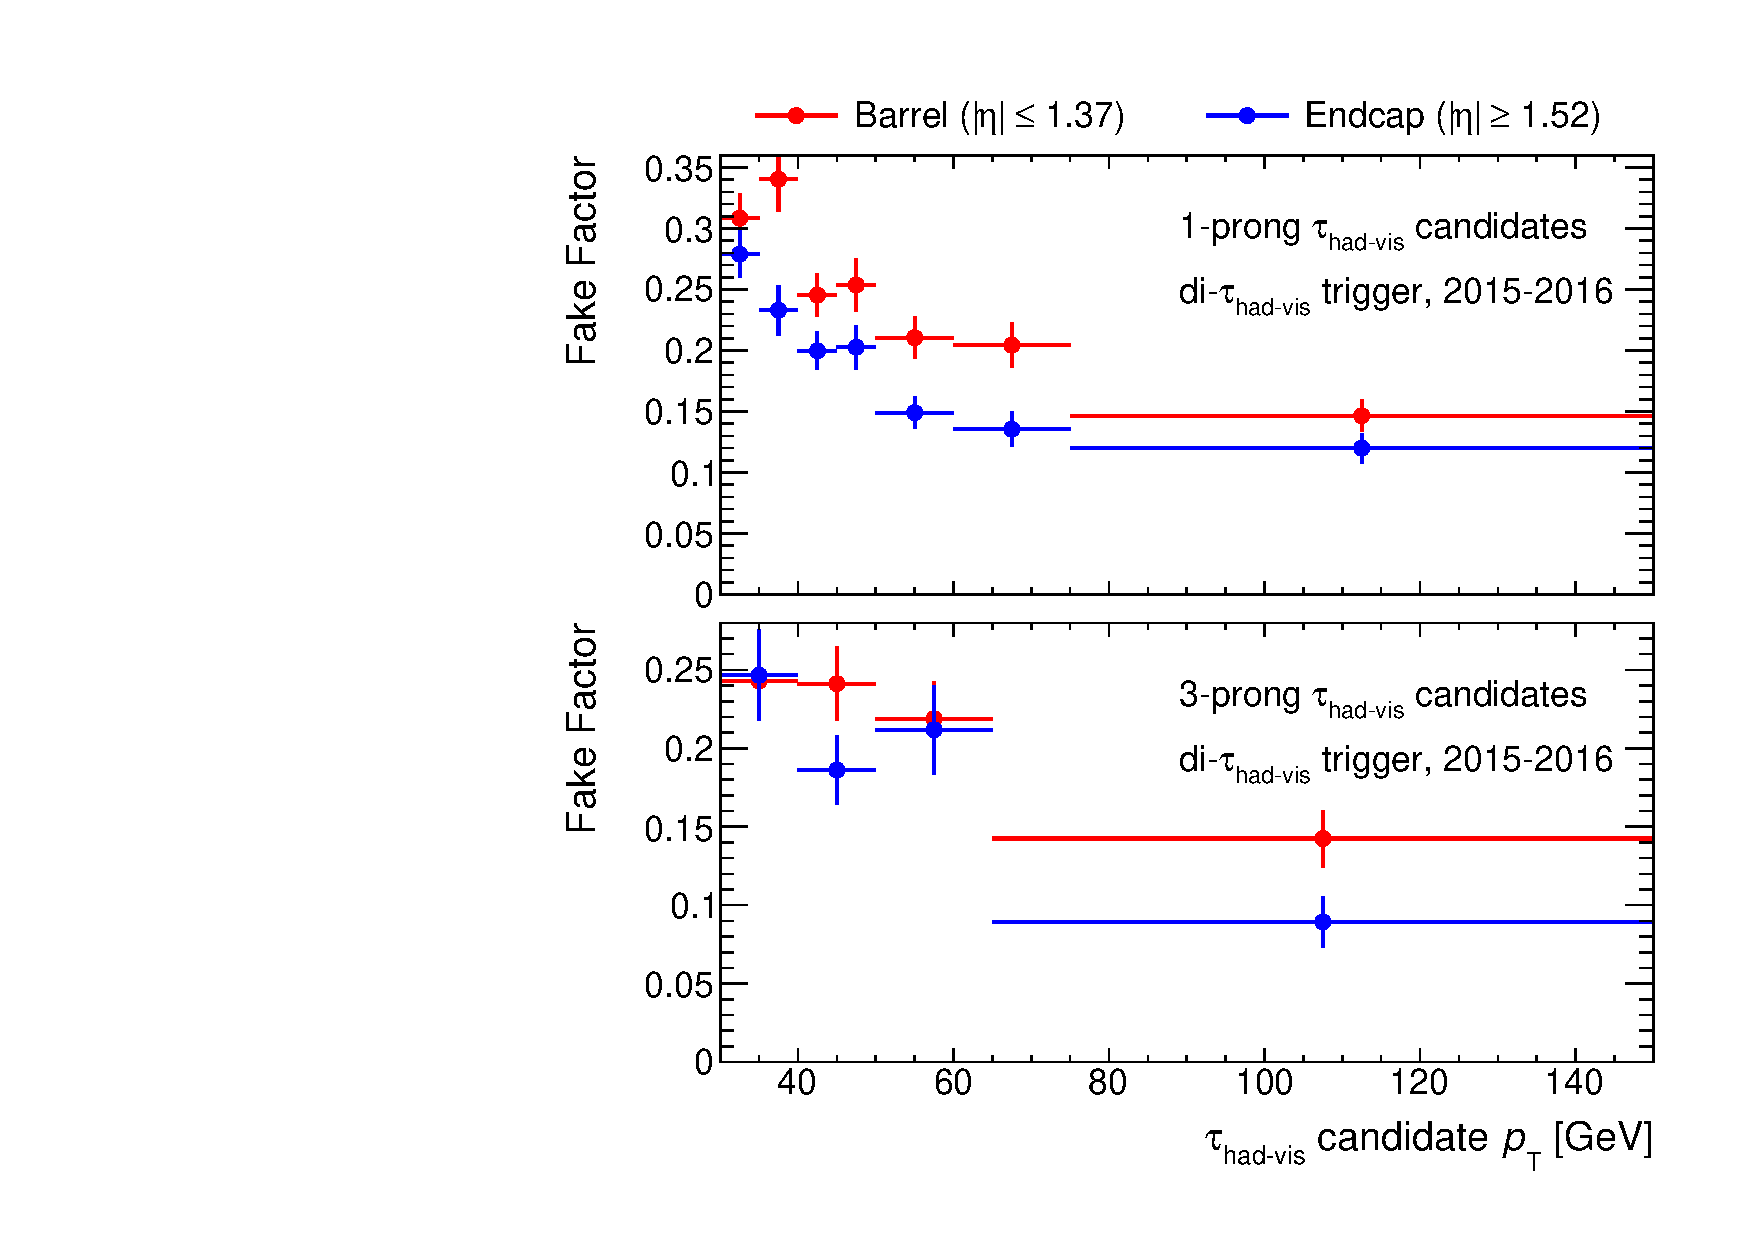
\includegraphics[width=\textwidth]{fakefactors/fake_factors_dtt_1516}
    \subcaption{2015-2016 data collection period}
  \end{subfigure}
  \begin{subfigure}{0.495\textwidth}
    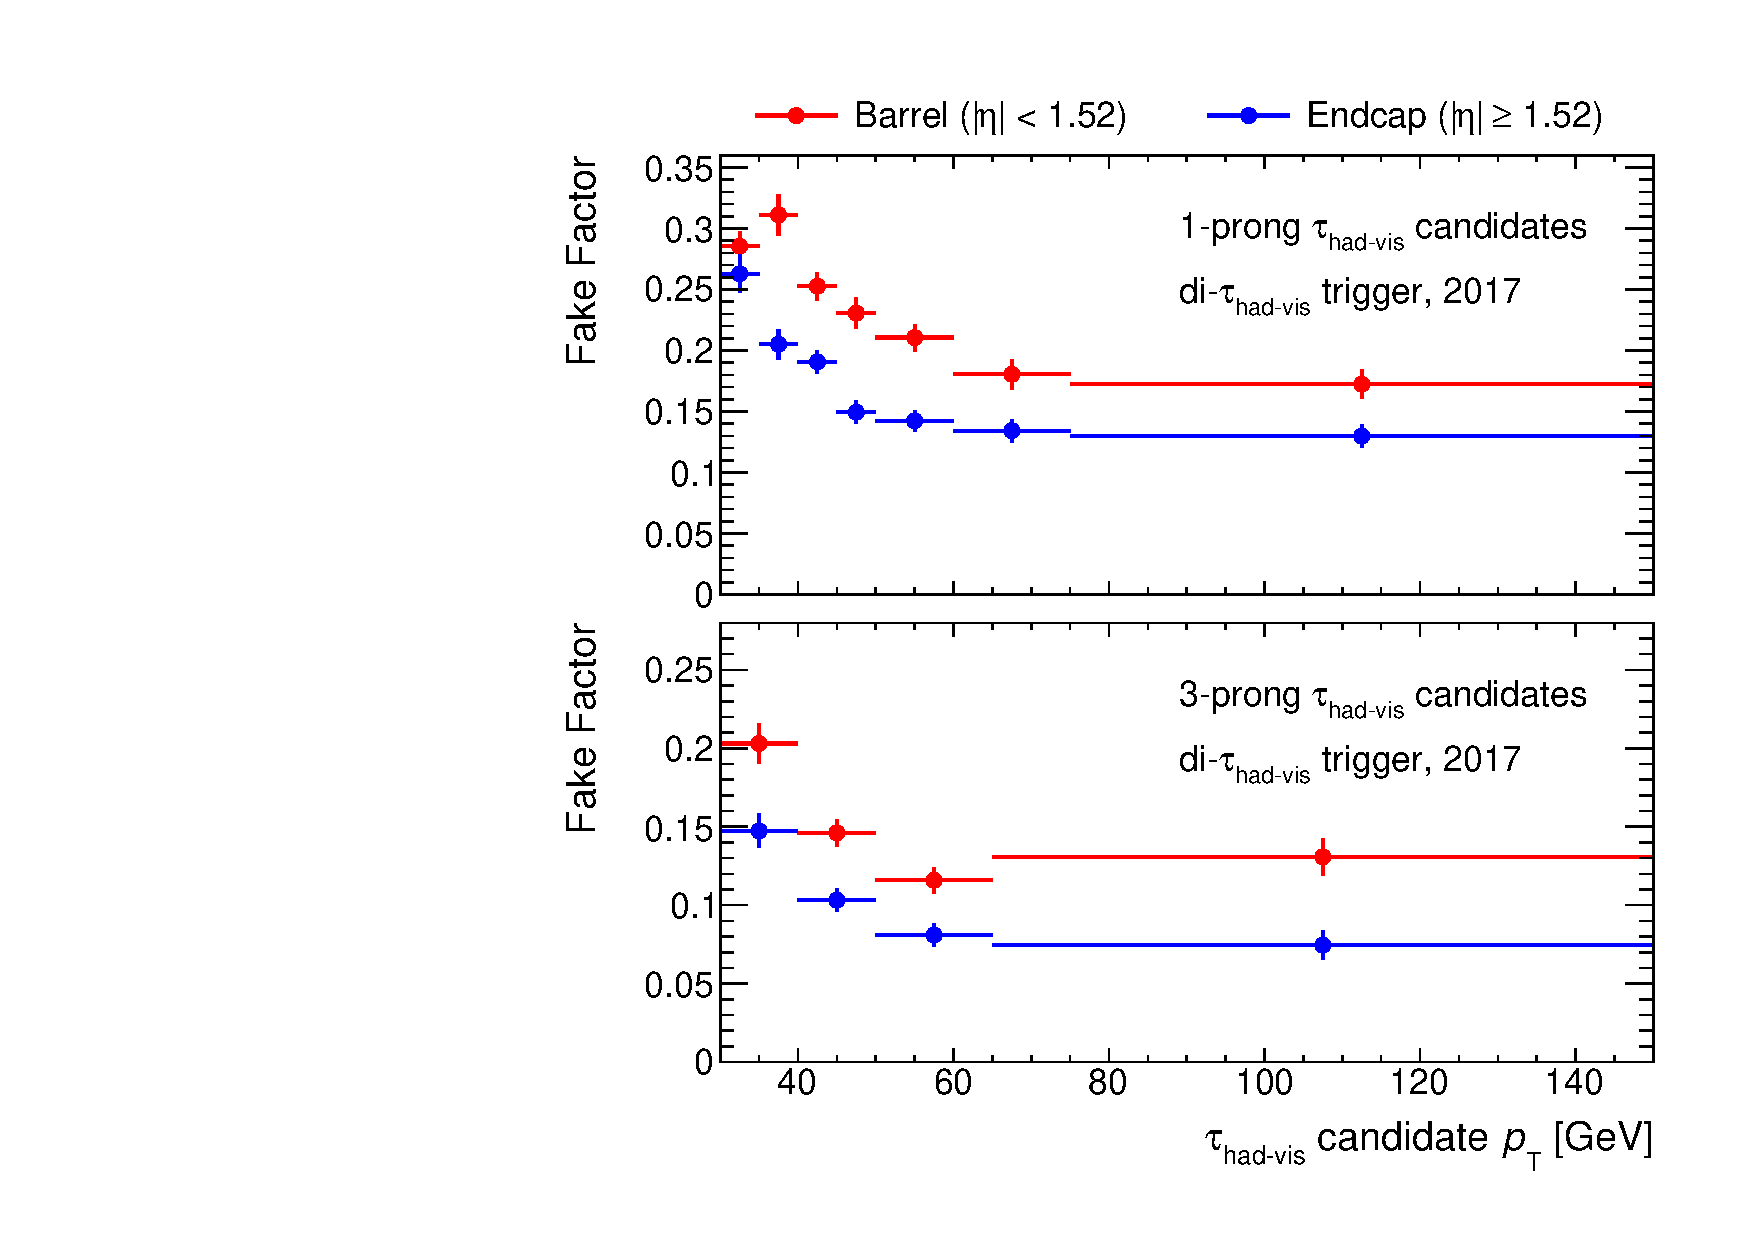
\includegraphics[width=\textwidth]{fakefactors/fake_factors_dtt_17}
    \subcaption{2017 data collection period}
  \end{subfigure}

  \begin{subfigure}{0.495\textwidth}
    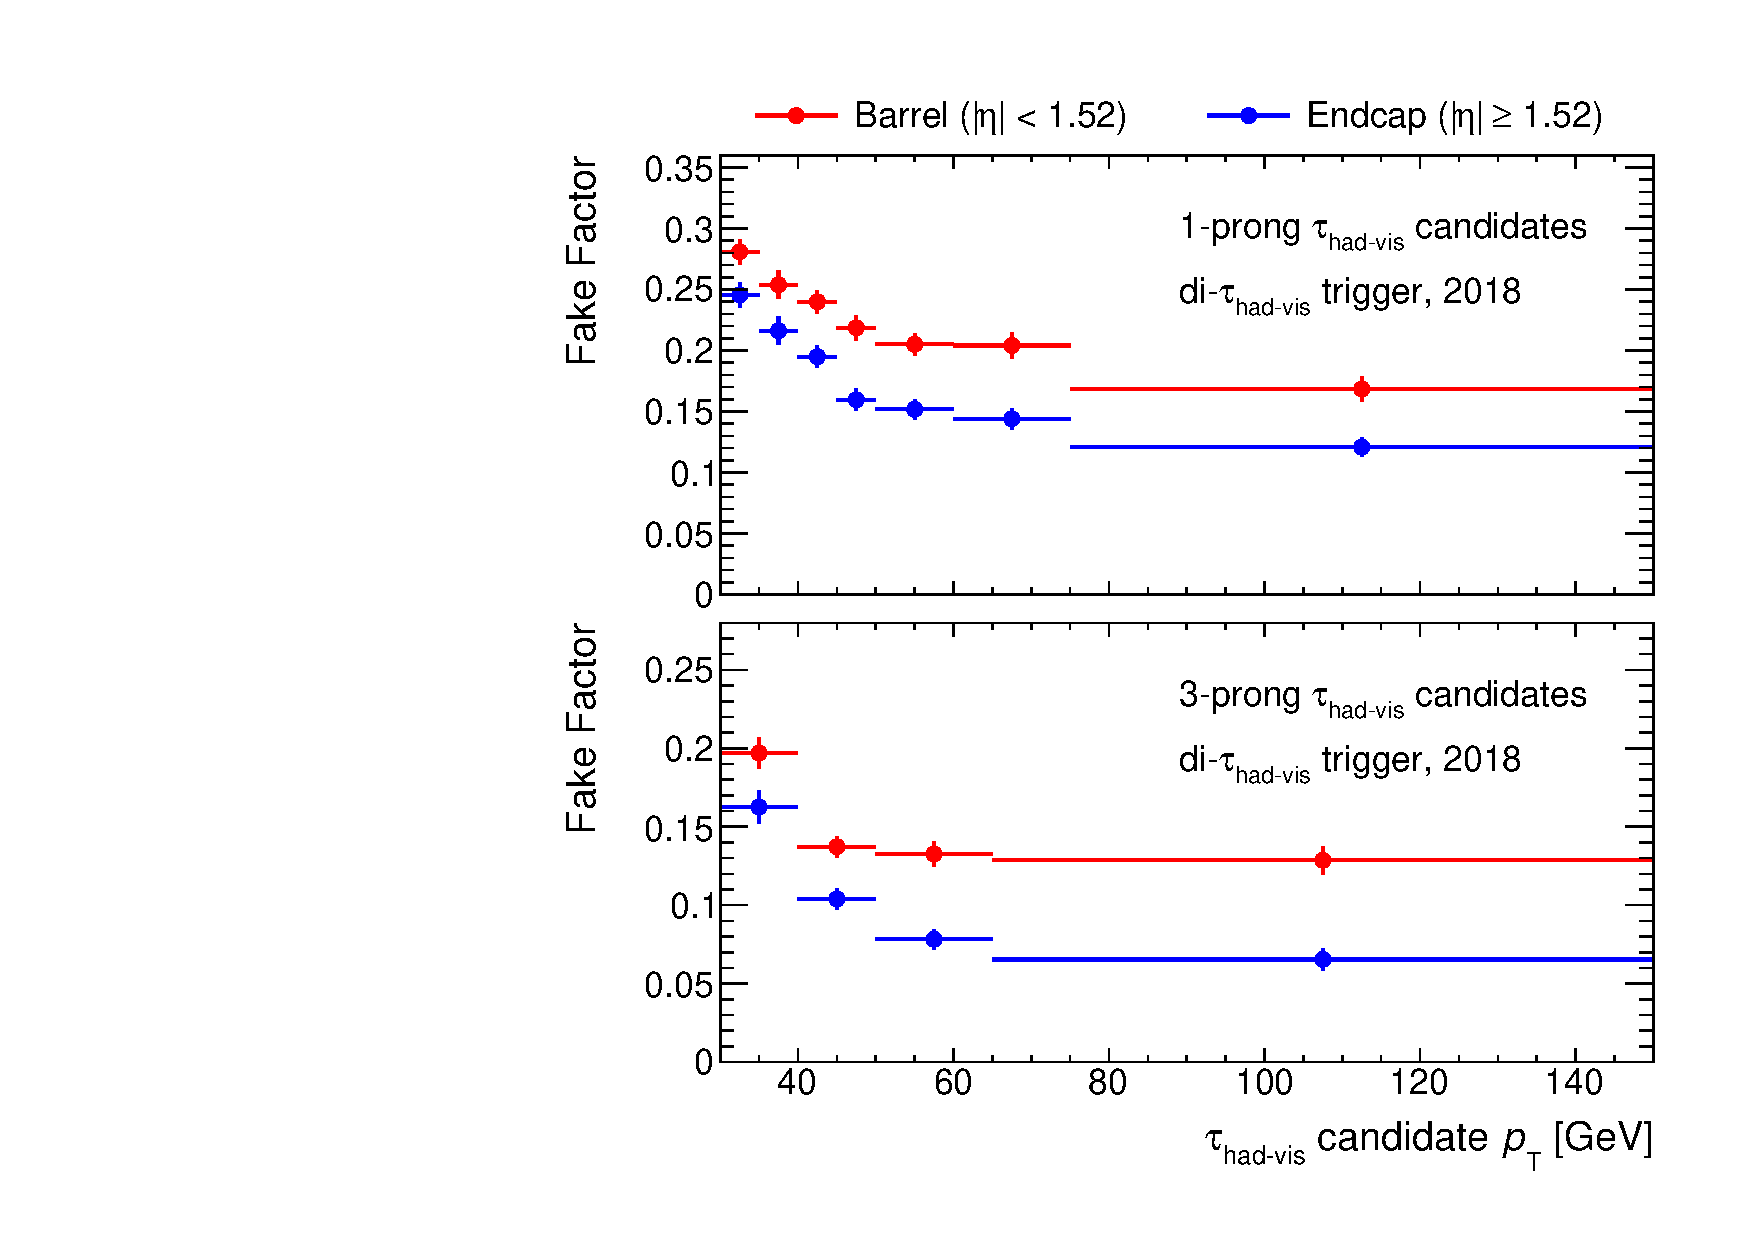
\includegraphics[width=\textwidth]{fakefactors/fake_factors_dtt_18}
    \subcaption{2018 data collection period}
  \end{subfigure}

  \caption{Inclusive fake factors for events selected by di-\tauhadvis
    triggers measured in the 1 $b$-tag SS region. The measurement is
    performed separately for the three major data collection periods
    (a-c), 1- and 3-prong \tauhadvis candidates (upper / lower
    panels), and for \tauhadvis in the barrel (red) and endcap regions
    (blue) of the ATLAS detector. Events with (anti-)\tauhadvis
    $\pT > \SI{150}{\GeV}$ are included in the last fake factor
    bin. Uncertainties are from statistical sources only. Systematic
    uncertainties originating from the non-multi-jet subtraction are
    assumed to be negligible due to the small size of the subtraction
    in the 1 $b$-tag SS region.}
  \label{fig:mjfakes_fake_factors}
\end{figure}


\subsubsection{Measurement of fake factors: single-\tauhadvis
  triggers}

The measurement of fake factors for events selected by
single-\tauhadvis triggers proceeds differently from the di-\tauhadvis
trigger case. Due to the selections applied at the HLT and the usually
large difference in \pT between both \tauhadvis candidates, the
single-\tauhadvis trigger fake factors are measured separately for the
leading and sub-leading \tauhadvis candidates. Additionally, the high
\pT thresholds on \tauhadvis at trigger-level provide large rejection
of most SM processes, limiting the number of events entering the
control regions for the fake factor measurement, thus preventing a
differential fake factor measurement in \tauhadvis \pT and $\eta$.

The approach of averaging the background estimates obtained from the
two partitions of the Anti-ID region remains valid for
single-\tauhadvis triggers, including~\Cref{eq:inclusive_fake_factor}
which can be used to calculate the fake factors. The main difference
between the the single- and di-\tauhadvis trigger fake factor
measurement is the replacement of the variables specifying the \pT and
$\eta$ bin in $\myvec{x}_\tau$ with an indicator variable specifying
whether the anti-\tauhadvis is leading or sub-leading in \pT.

% First, at the HLT \tauhadvis
% identification is only applied to one of the \tauhadvis candidates,
% preventing an inclusive treatment of both \tauhadvis
% candidates. Second, the high \pT thresholds on \tauhadvis at
% trigger-level has high rejection of most SM processes, limiting the
% number of events entering the control regions for the fake factor
% measurement. As a result, the fake factors for singe-\tauhadvis
% triggers cannot be measured differentially in \tauhadvis \pT and
% $\eta$.

The measured single-\tauhadvis trigger fake factors are shown
in~\Cref{fig:mjfakes_stt_ffs} for the three major data collection
periods. Each period is divided into four categories depending on
$N_{\text{tracks}}$ and whether the anti-\tauhadvis is leading
($\tau_0$) or sub-leading ($\tau_1$) in \pT.

\begin{figure}[htbp]
  \centering

  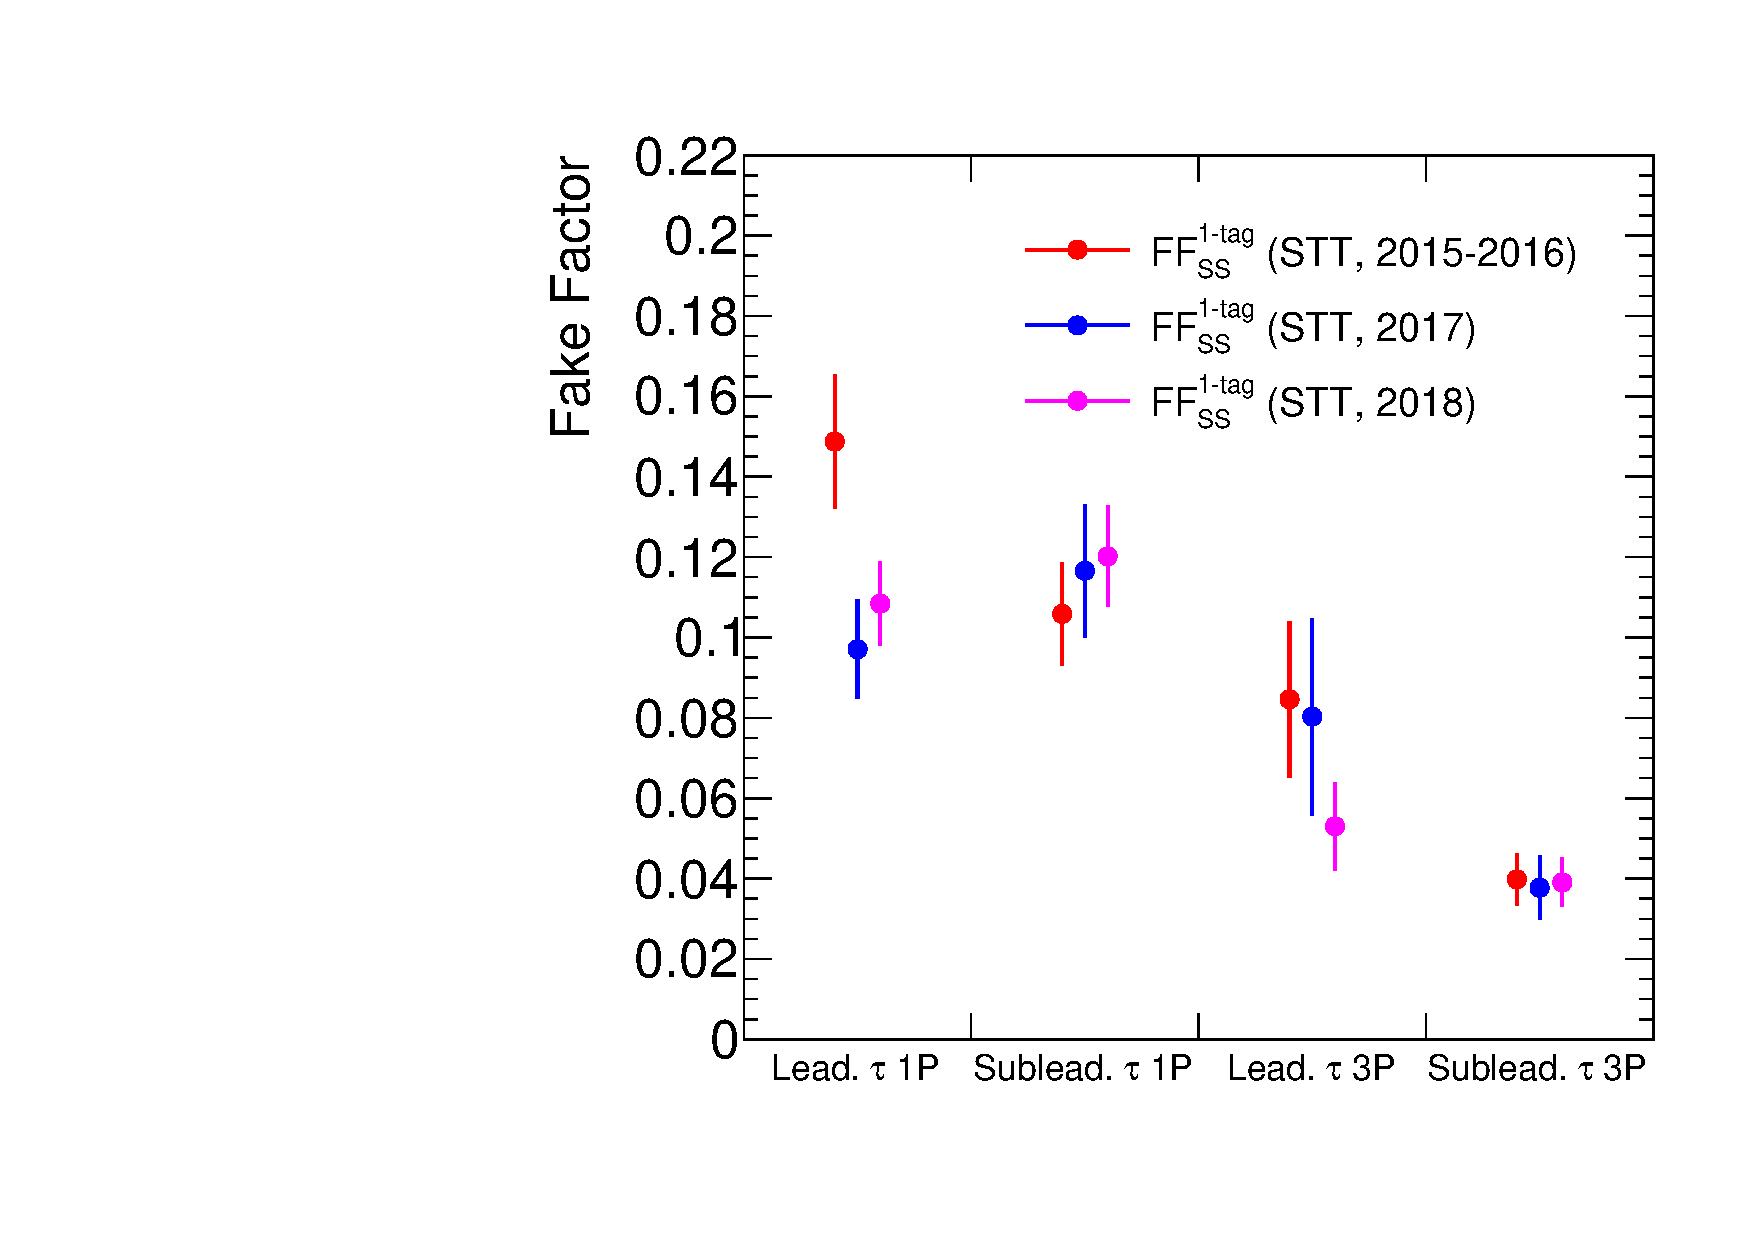
\includegraphics[width=0.495\textwidth]{fakefactors/fake_factors_stt}

  \caption{Single-\tauhadvis trigger fake factors measured in the 1
    $b$-tag SS region, separately for the three major data collection
    periods. The measurement is performed in bins of the reconstructed
    \tauhadvis decay mode (1- and 3-prong) and separately for cases
    where the anti-\tauhadvis is leading ($\tau_0$) and sub-leading in
    \pT ($\tau_1$).}%
  \label{fig:mjfakes_stt_ffs}
  % \todo[inline]{Largest deviation for leading 1-prong tau possibly
  % due to looser pT threshold.}
\end{figure}


\subsubsection{Validation of the multi-jet estimate in the 1 $b$-tag OS region}

An independent validation of the background estimate can be performed
in the 1 $b$-tag OS ID region (cf.\ \Cref{fig:fakefactor_regions}).
% , which is not part of the fake factor measurement.
At pre-selection level this region has a multi-jet purity of ca.\
\SI{50}{\percent} with the dominant non-multi-jet contributions
originating from \Zjets and \ttbar. The multi-jet purity is enhanced
for validation purposes by requiring events to fulfil
% https://twiki.cern.ch/twiki/bin/view/AtlasProtected/MetSignificance
% Using `TreatPUJets == true' and Basic soft term (met::Random)
\begin{align*}
  \mMMC > \SI{110}{\GeV} \qquad \text{and} \qquad \mathcal{S} < 3 \,\text{,}
\end{align*}
where $\mathcal{S}$ is the object-based \pTmissAbs
significance~\cite{ATLAS-CONF-2018-038}. The \pTmissAbs significance
measures the statistical significance of a test comparing the
hypothesis that the reconstructed \pTmissAbs is compatible with zero
within the expected measurement errors, to the alternative hypothesis
of \pTmissAbs primarily originating from undetected weakly interacting
particles.

The variables used to define the multi-jet validation region are shown
in~\Cref{fig:fake_factor_OSVR_cutvars} after pre-selection. The
contribution of \Zjets is reduced by rejecting events with
di-$\tauhad$ masses close to the \PZ boson mass.  Multi-jet events are
expected to have little real \pTmissAbs, thus events with a
significant \pTmissAbs measurement are rejected to reduce the \ttbar
contribution in this region. The selection increases the multi-jet
purity in the validation region to \SI{75}{\percent} with a multi-jet
selection efficiency of about \SI{50}{\percent} with respect to the
pre-selection.

\begin{figure}[htbp]
  \centering

  \begin{subfigure}{0.45\textwidth}
    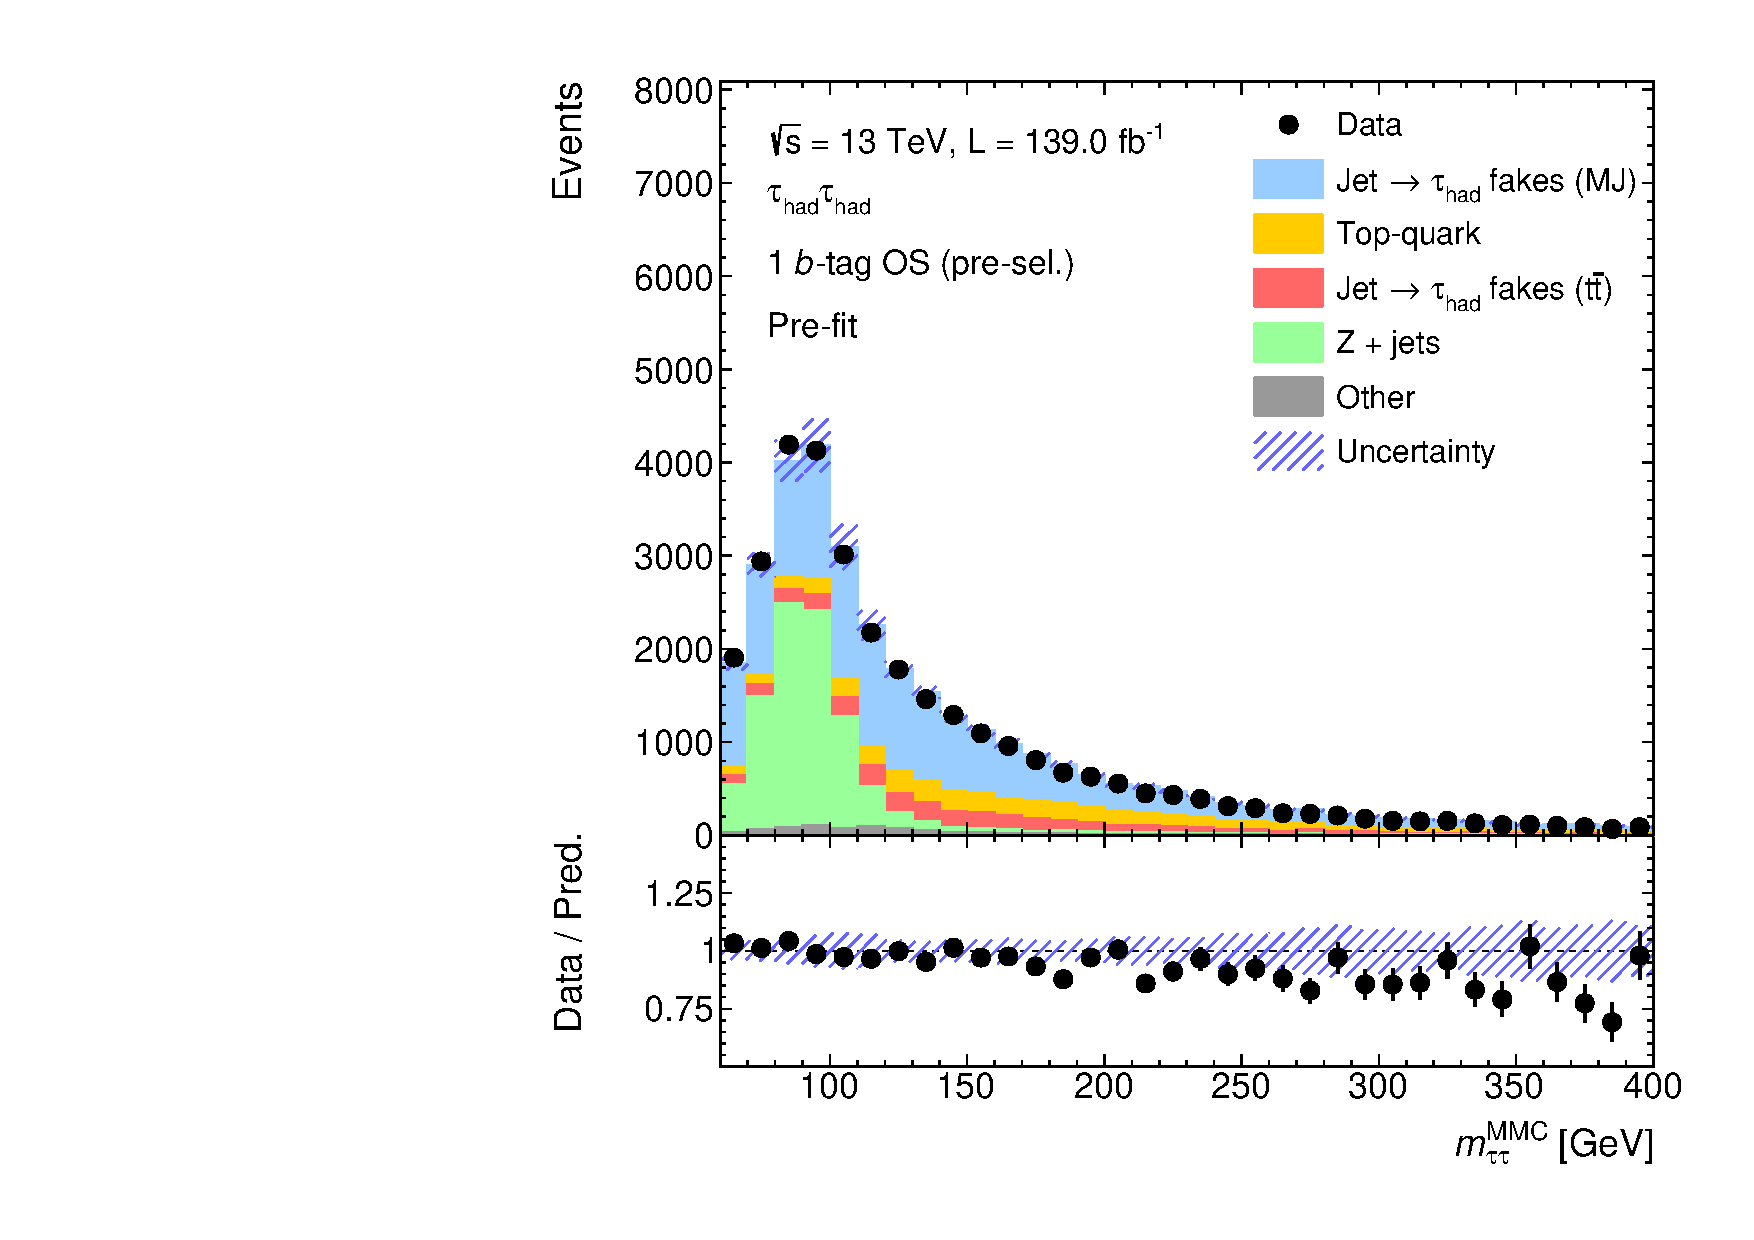
\includegraphics[width=\textwidth]{fakefactors/fake_os_vr/mMMC_presel}
    \subcaption{}
  \end{subfigure}\hspace*{0.04\textwidth}%
  \begin{subfigure}{0.45\textwidth}
    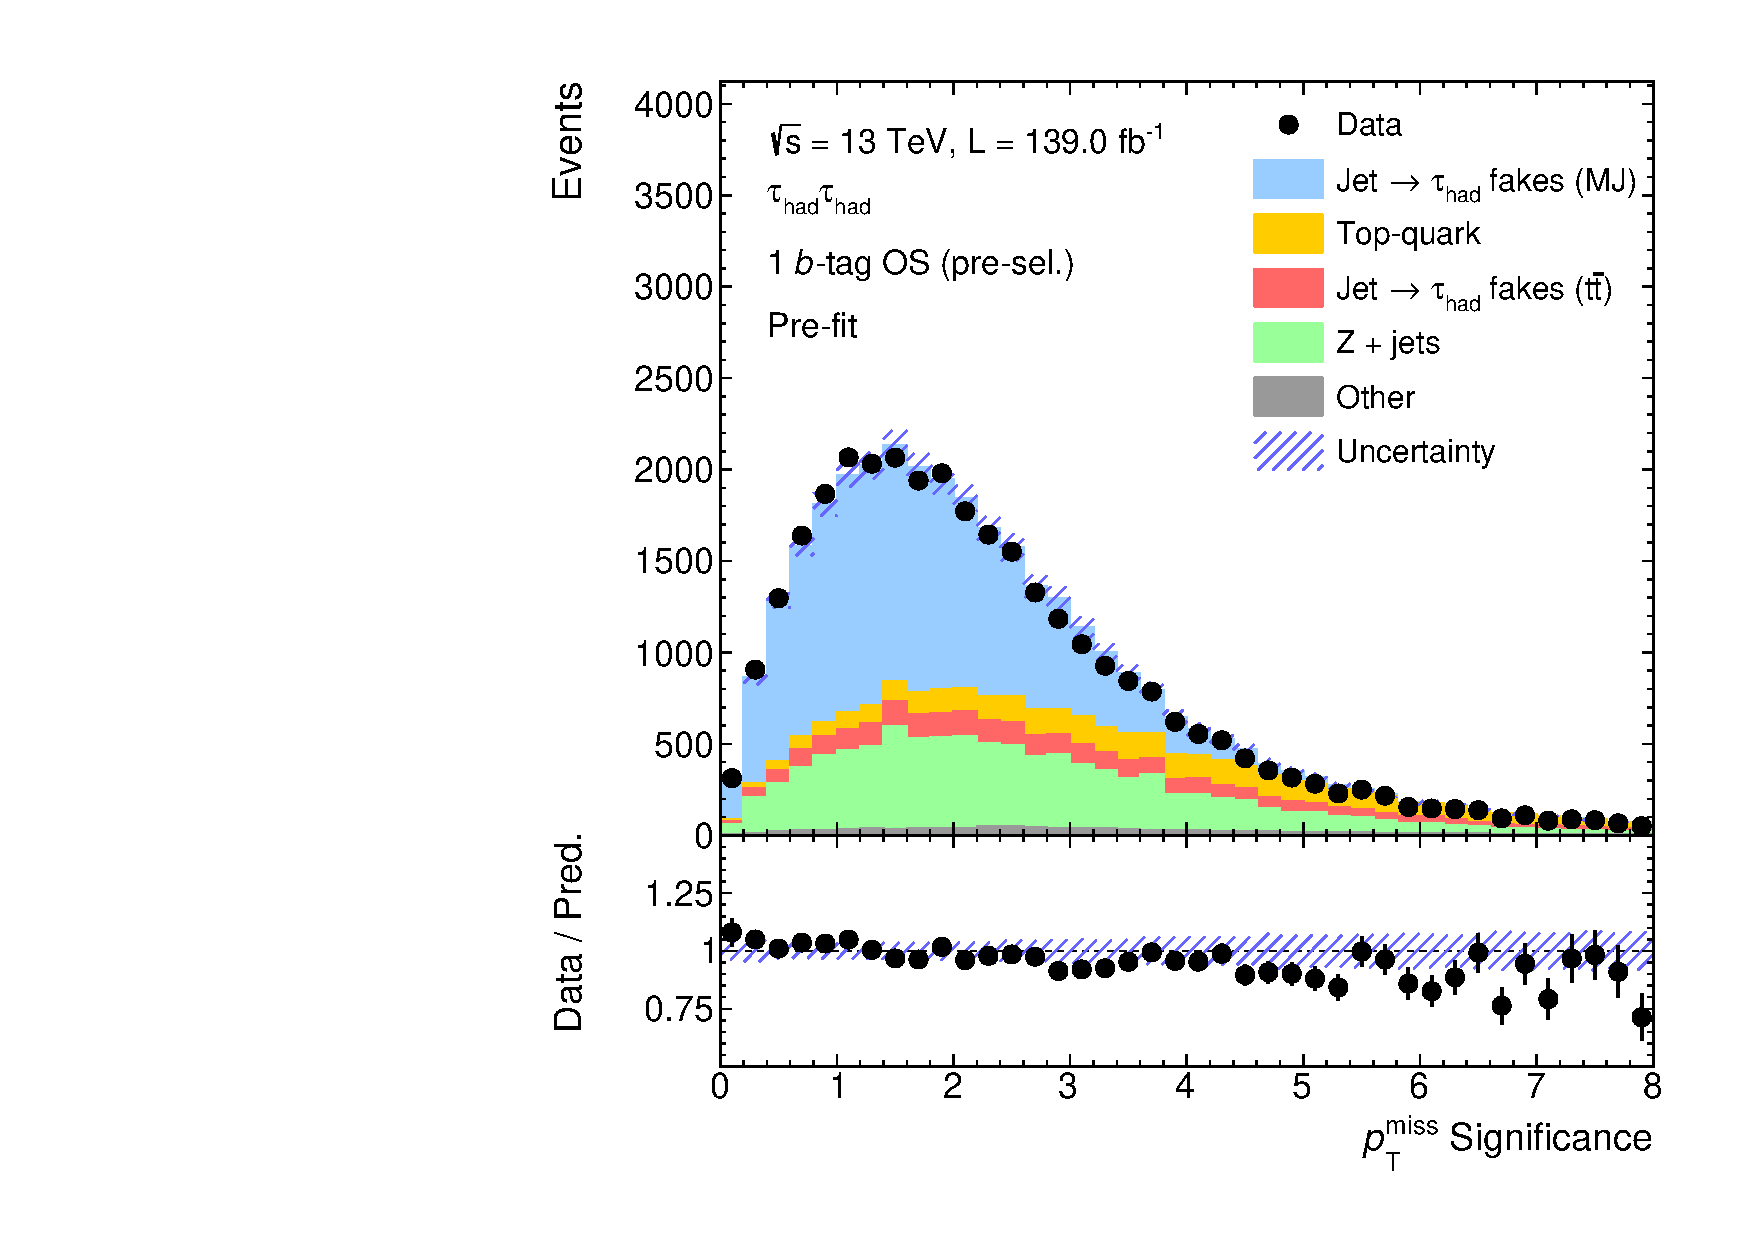
\includegraphics[width=\textwidth]{fakefactors/fake_os_vr/metSig_presel}
    \subcaption{}
  \end{subfigure}

  \caption{The invariant di-\tauhad mass (a) and the object-based
    \pTmissAbs significance (b) in the 1 $b$-tag OS ID region after
    the pre-selection. The estimate of the multi-jet background (light
    blue) is obtained using the fake factor method (cf.\
    \Cref{fig:fakefactor_regions}). Fake-\tauhadvis originating from
    \ttbar (red) are estimated using simulation. The background
    prediction is shown pre-fit, including statistical and
    detector-related systematic uncertainties.}
  \label{fig:fake_factor_OSVR_cutvars}
\end{figure}

The multi-jet background prediction in the validation region is
obtained by applying the measured fake factors to events in the OS
Anti-ID region after subtracting non-multi-jet contributions. The
non-multi-jet backgrounds in the OS ID region are estimated using
simulation. The total background prediction in the multi-jet VR is
compared to data in~\Cref{fig:fake_factor_OSVR_kinematics} for several
observables of the leading and sub-leading \tauhadvis candidate.

\begin{figure}[htbp]
  \centering

  \begin{subfigure}{0.45\textwidth}
    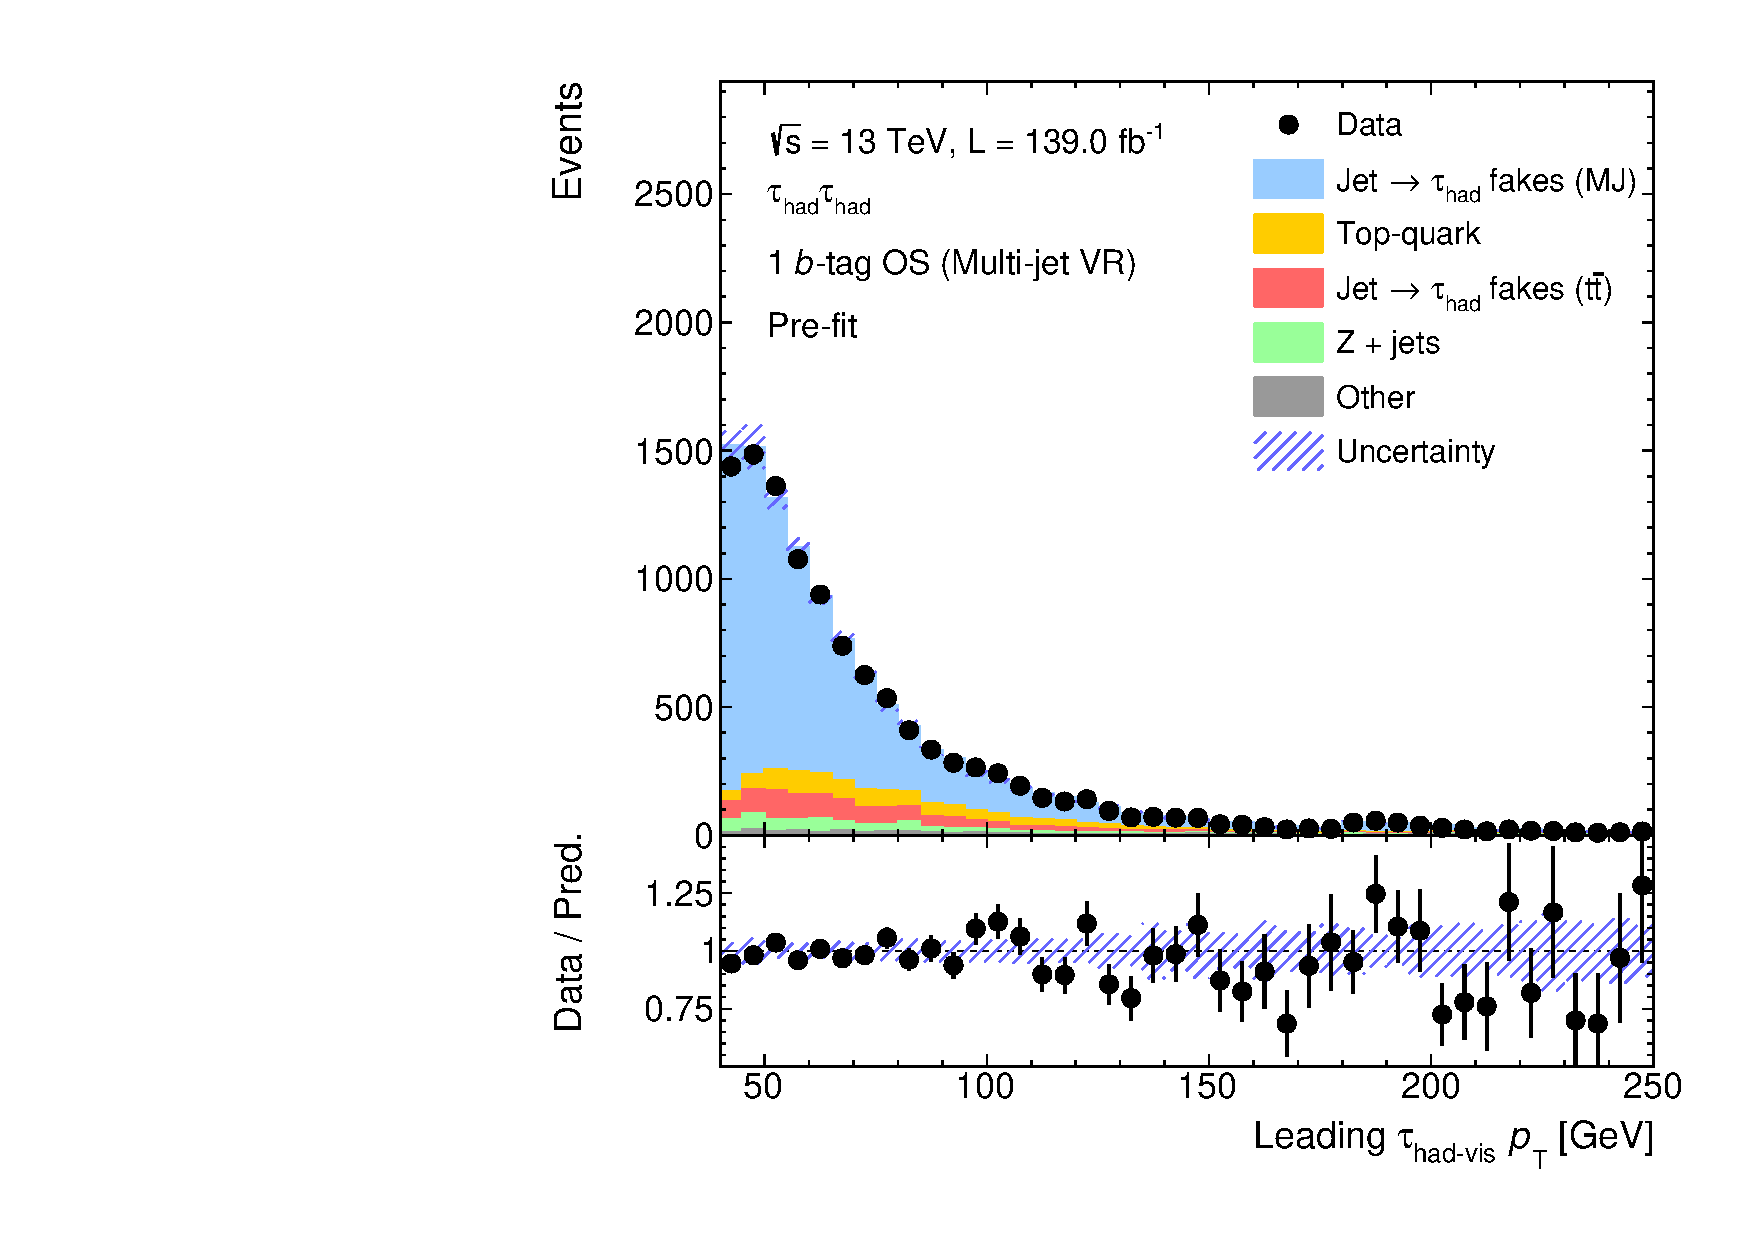
\includegraphics[width=\textwidth]{fakefactors/fake_os_vr/Tau0Pt_fakevr}
  \end{subfigure}\hspace*{0.04\textwidth}%
  \begin{subfigure}{0.45\textwidth}
    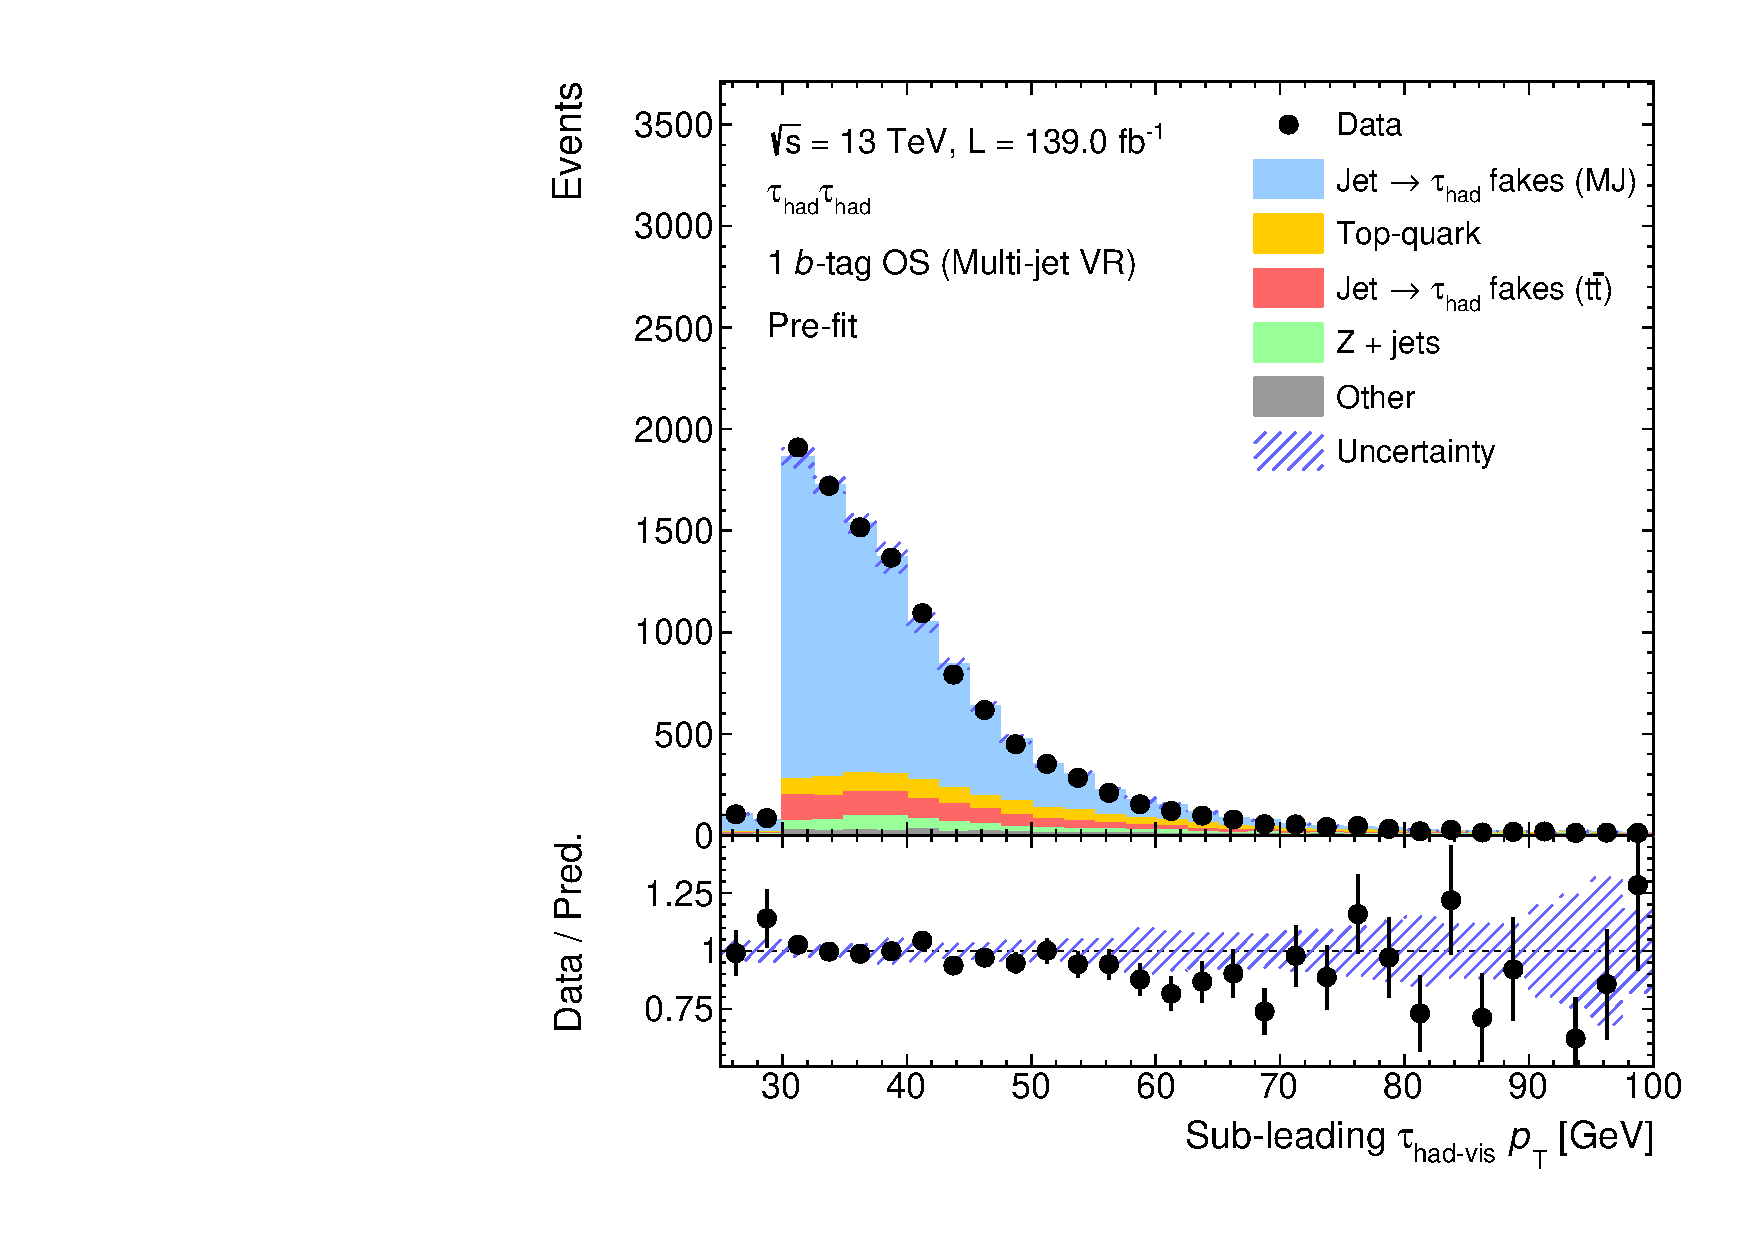
\includegraphics[width=\textwidth]{fakefactors/fake_os_vr/Tau1Pt_fakevr}
  \end{subfigure}

  \begin{subfigure}{0.45\textwidth}
    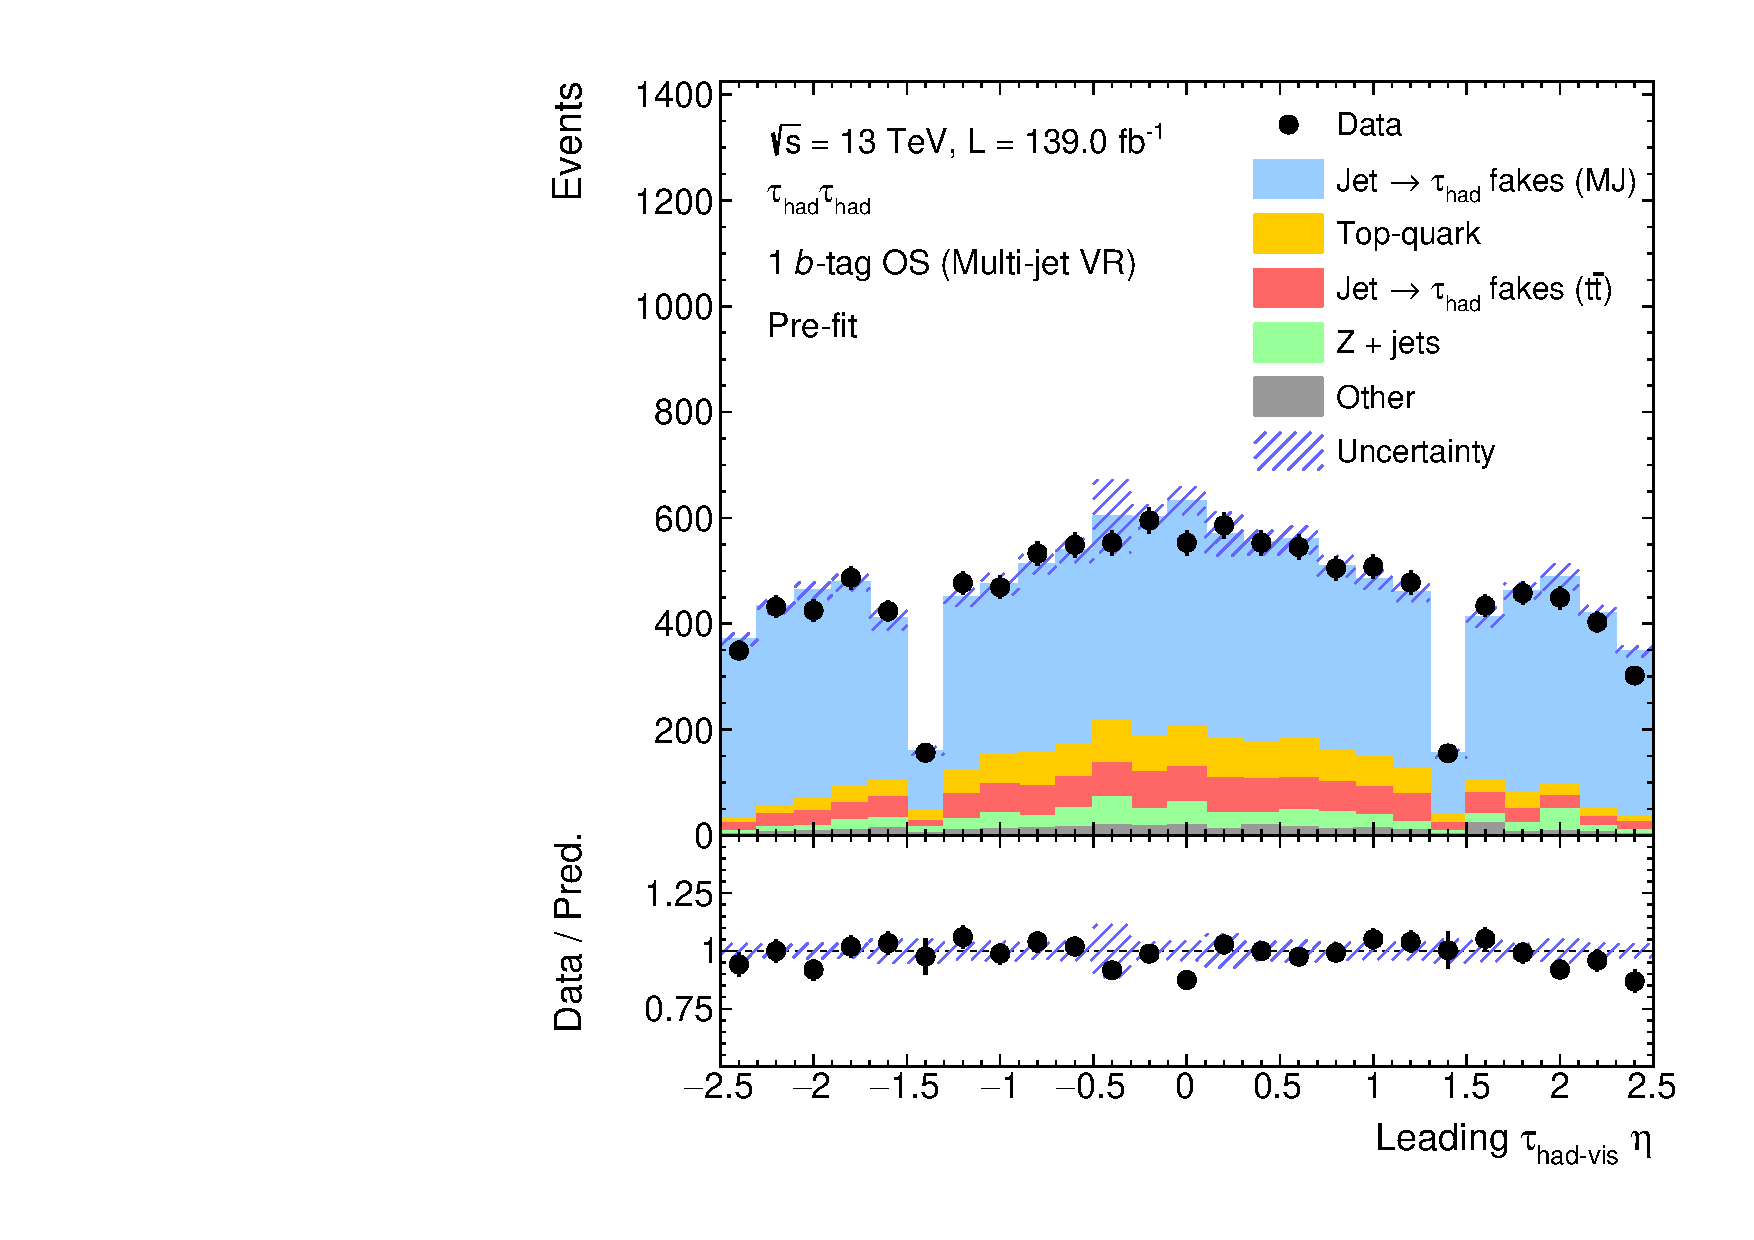
\includegraphics[width=\textwidth]{fakefactors/fake_os_vr/Tau0Eta_fakevr}
  \end{subfigure}\hspace*{0.04\textwidth}%
  \begin{subfigure}{0.45\textwidth}
    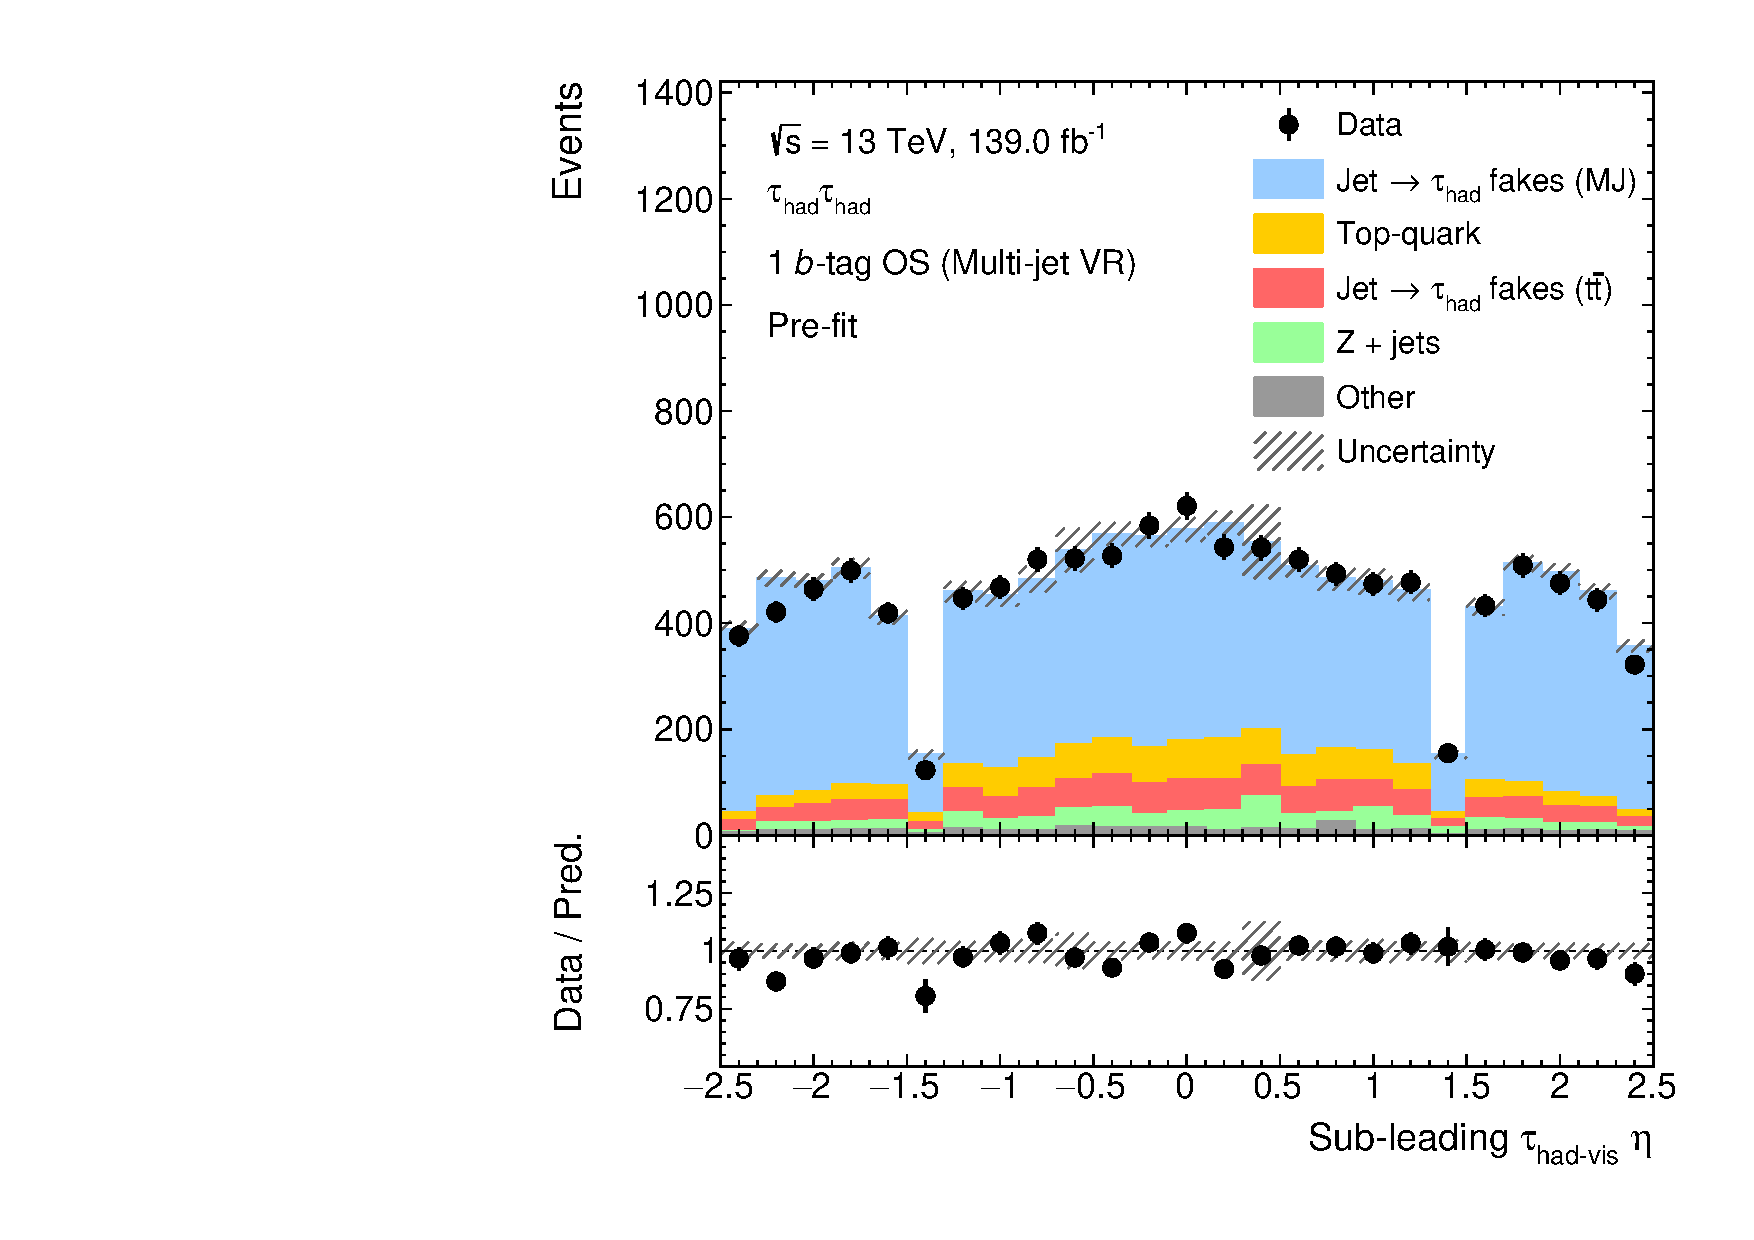
\includegraphics[width=\textwidth]{fakefactors/fake_os_vr/Tau1Eta_fakevr}
  \end{subfigure}

  \begin{subfigure}{0.45\textwidth}
    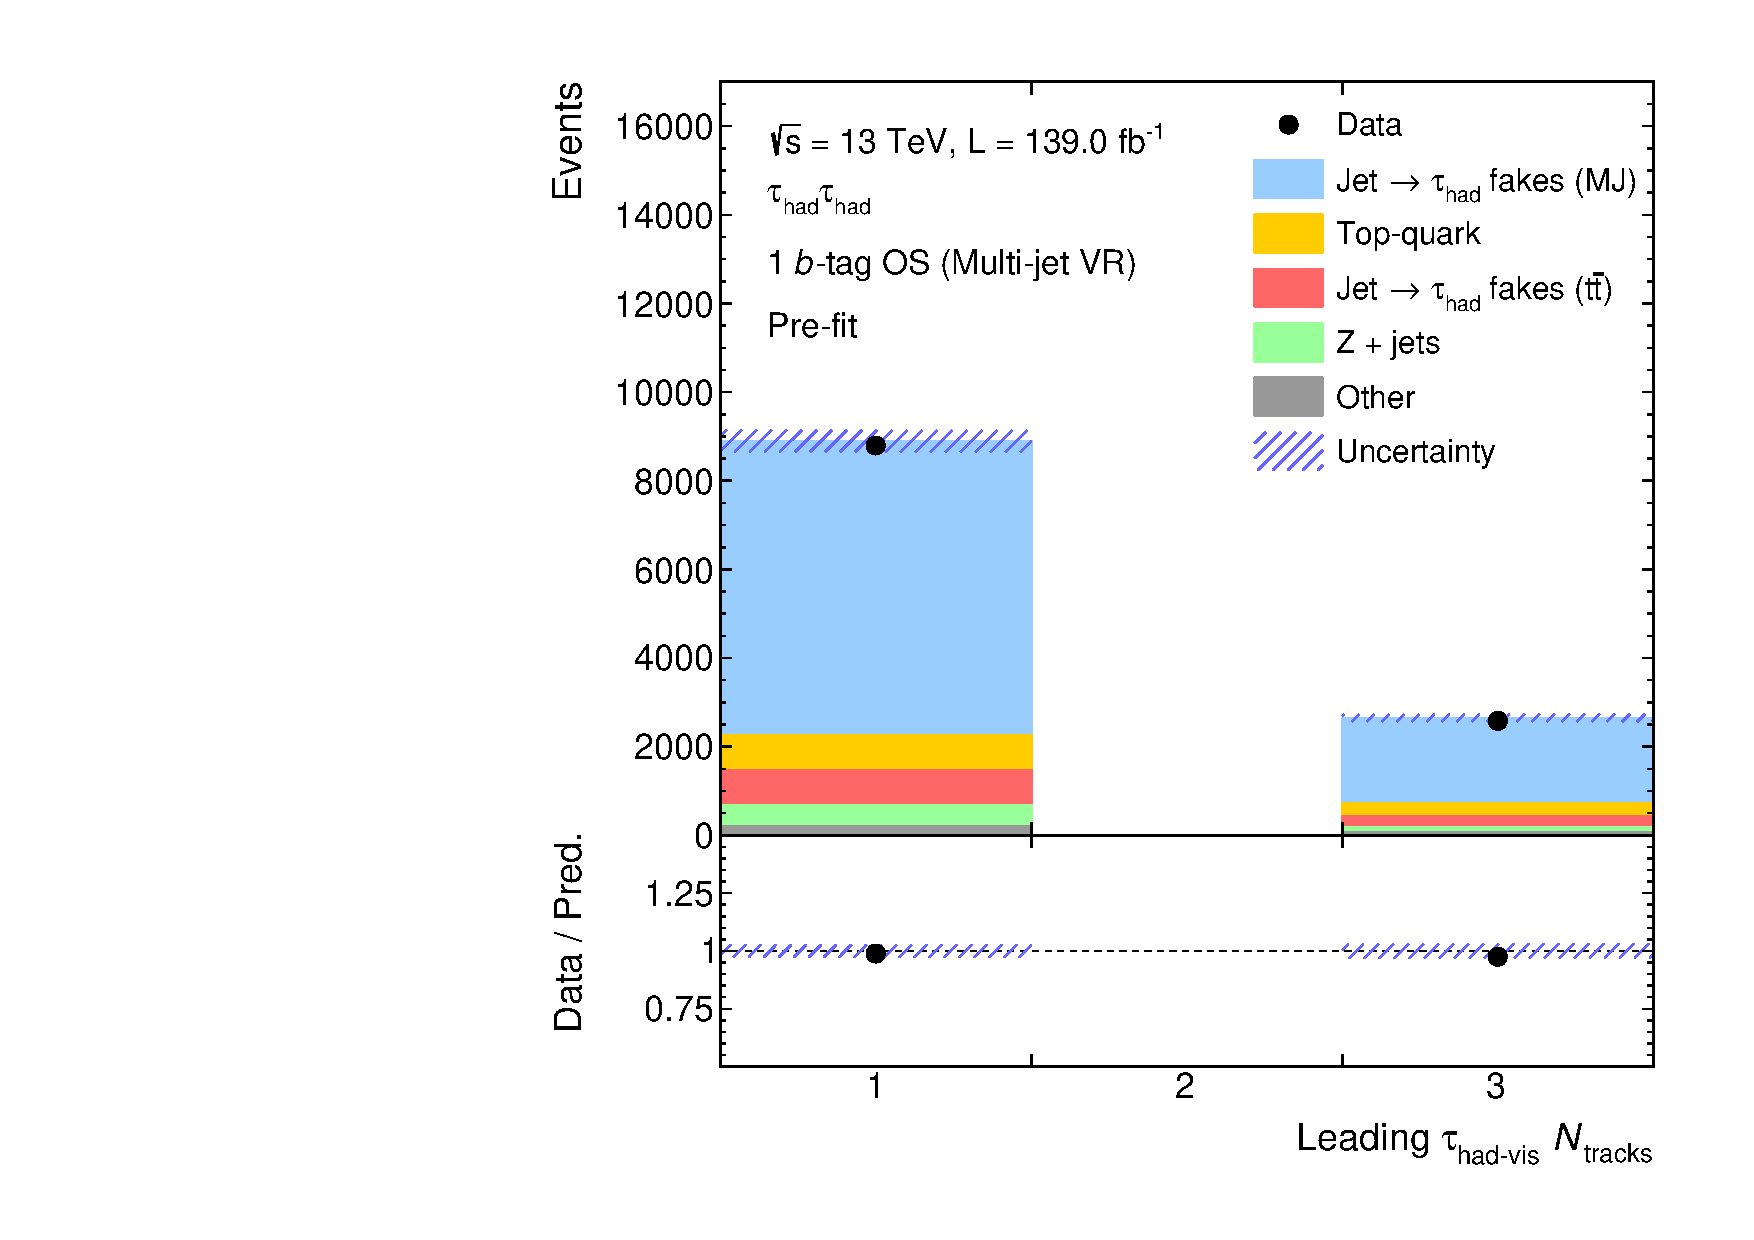
\includegraphics[width=\textwidth]{fakefactors/fake_os_vr/Tau0Ntrk_fakevr}
  \end{subfigure}\hspace*{0.04\textwidth}%
  \begin{subfigure}{0.45\textwidth}
    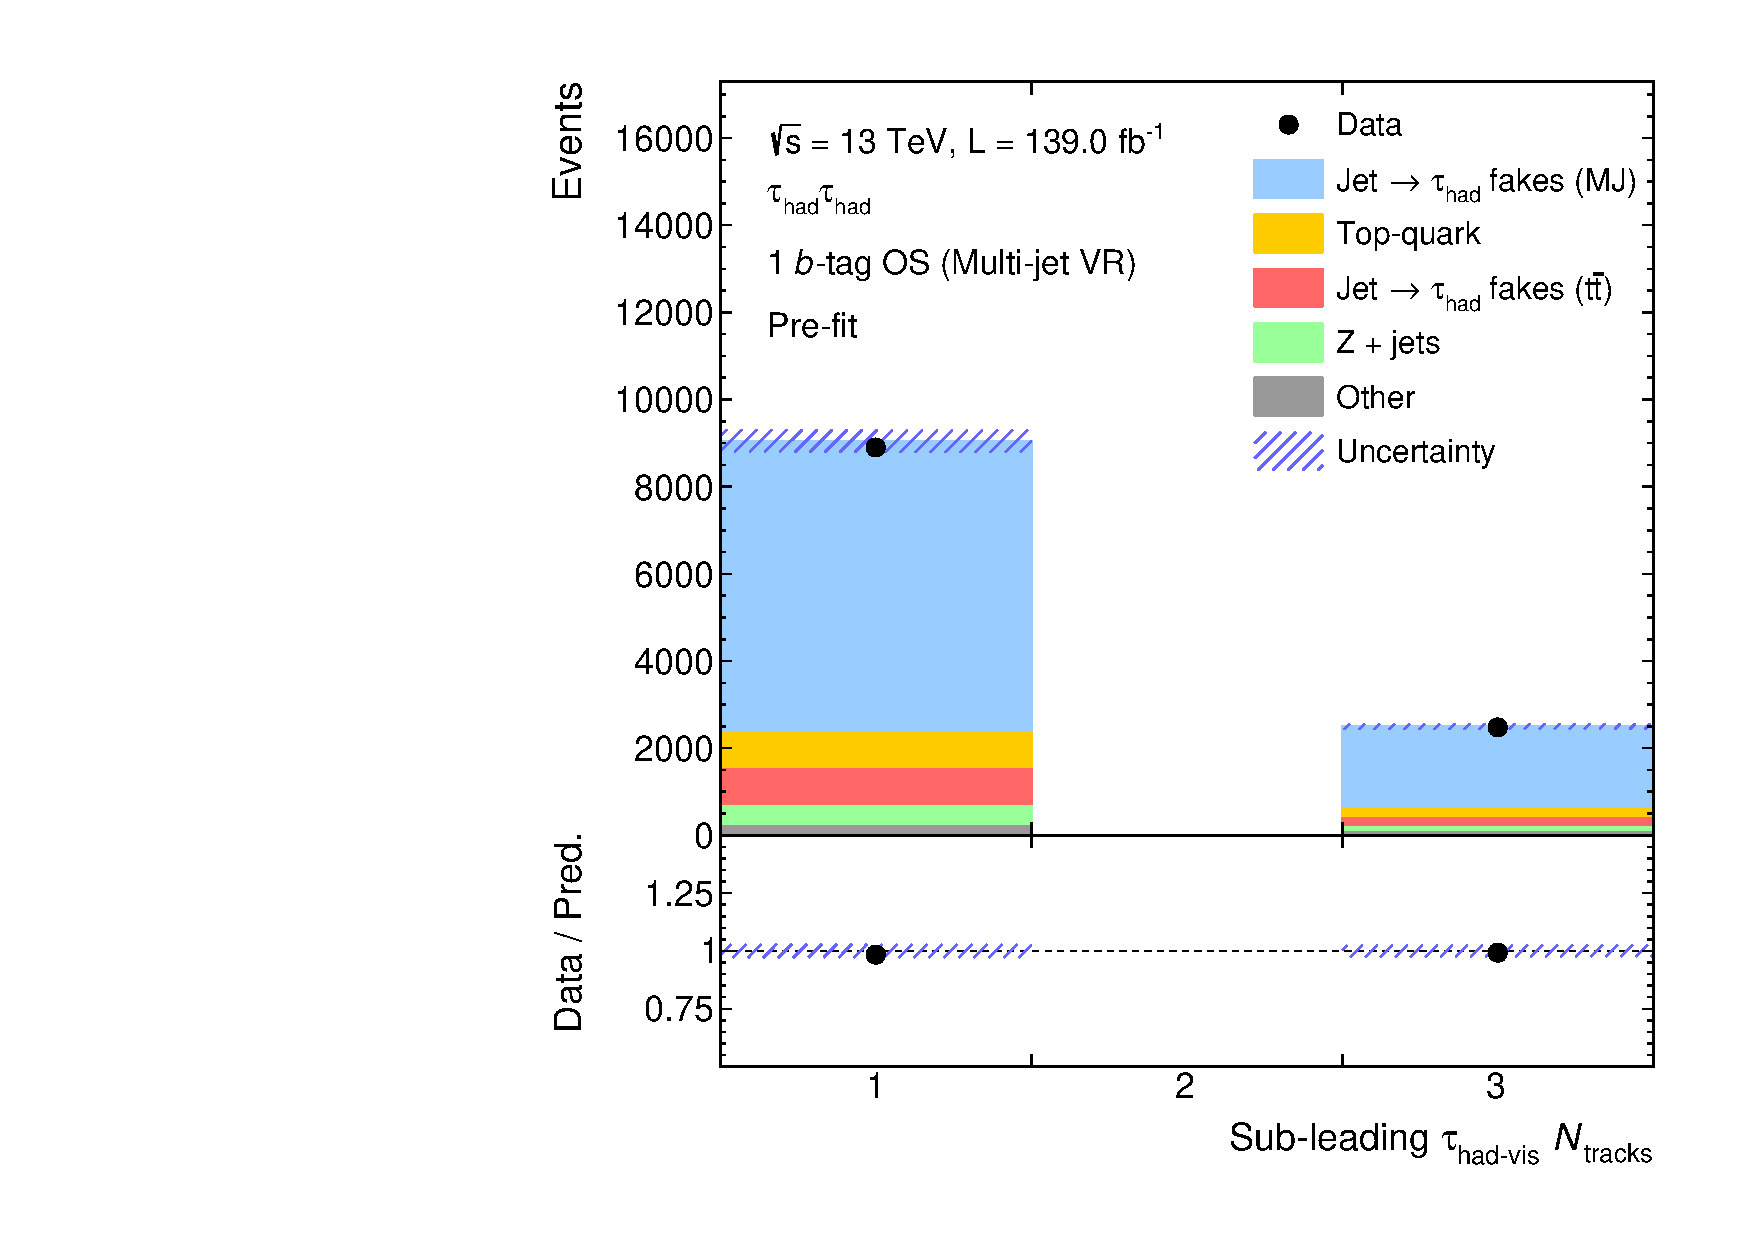
\includegraphics[width=\textwidth]{fakefactors/fake_os_vr/Tau1Ntrk_fakevr}
  \end{subfigure}

  \caption{Validation of \tauhadvis observables in the multi-jet VR
    defined by the requirements: 1 $b$-tag OS,
    $\mMMC > \SI{110}{\GeV}$, and $\mathcal{S} < 3$. The multi-jet
    background prediction (blue) is obtained using the fake factor
    method. The \tauhadvis observables \pT (top), $\eta$ (center), and
    $N_{\text{tracks}}$ (bottom) are shown for the leading (left) and
    sub-leading \tauhadvis (right). The background prediction is shown
    prior to the fit and includes statistical and detector-related
    systematic uncertainties.}%
  \label{fig:fake_factor_OSVR_kinematics}%
  % Explicitly say that there are no fake uncertainties here yet?
\end{figure}

Good agreement between the background prediction and data is observed
in the validation region for \tauhadvis-related observables. Further
tests of the assumptions of the fake factor method can be performed by
a comparison of the fake factors measured in the 1 $b$-tag SS region
with fake factors obtained from a measurement in the 1 $b$-tag OS
multi-jet VR. Under the assumptions of the fake factor method, both OS
and SS fake factors are expected to agree. Possible differences
between both sets of fake factors can originate from a violation of
the assumptions or from errors in the non-multi-jet subtraction.

The comparison of OS and SS fake factors is shown
in~\Cref{fig:fake_factor_OSSS} exemplary for di-\tauhadvis trigger
fake factors for the 2018 period and for all single-\tauhadvis trigger
fake factors. The fake factors are compared using $\chi^2$-tests
showing good agreement with one exception. A relative deviation of
\SI{50}{\percent} is observed for a single fake factor
bin\footnote{3-prong \tauhadvis with \pT from \SIrange{50}{65}{\GeV}
  in the endcap regions.} for di-\tauhadvis triggers in 2015-2016. To
account for the non-closure, the full difference between the central
values of OS and SS fake factors is assigned as a systematic
uncertainty and propagated to the multi-jet estimate.

\begin{figure}[htbp]
  \centering

  \begin{subfigure}[t]{0.48\textwidth}
    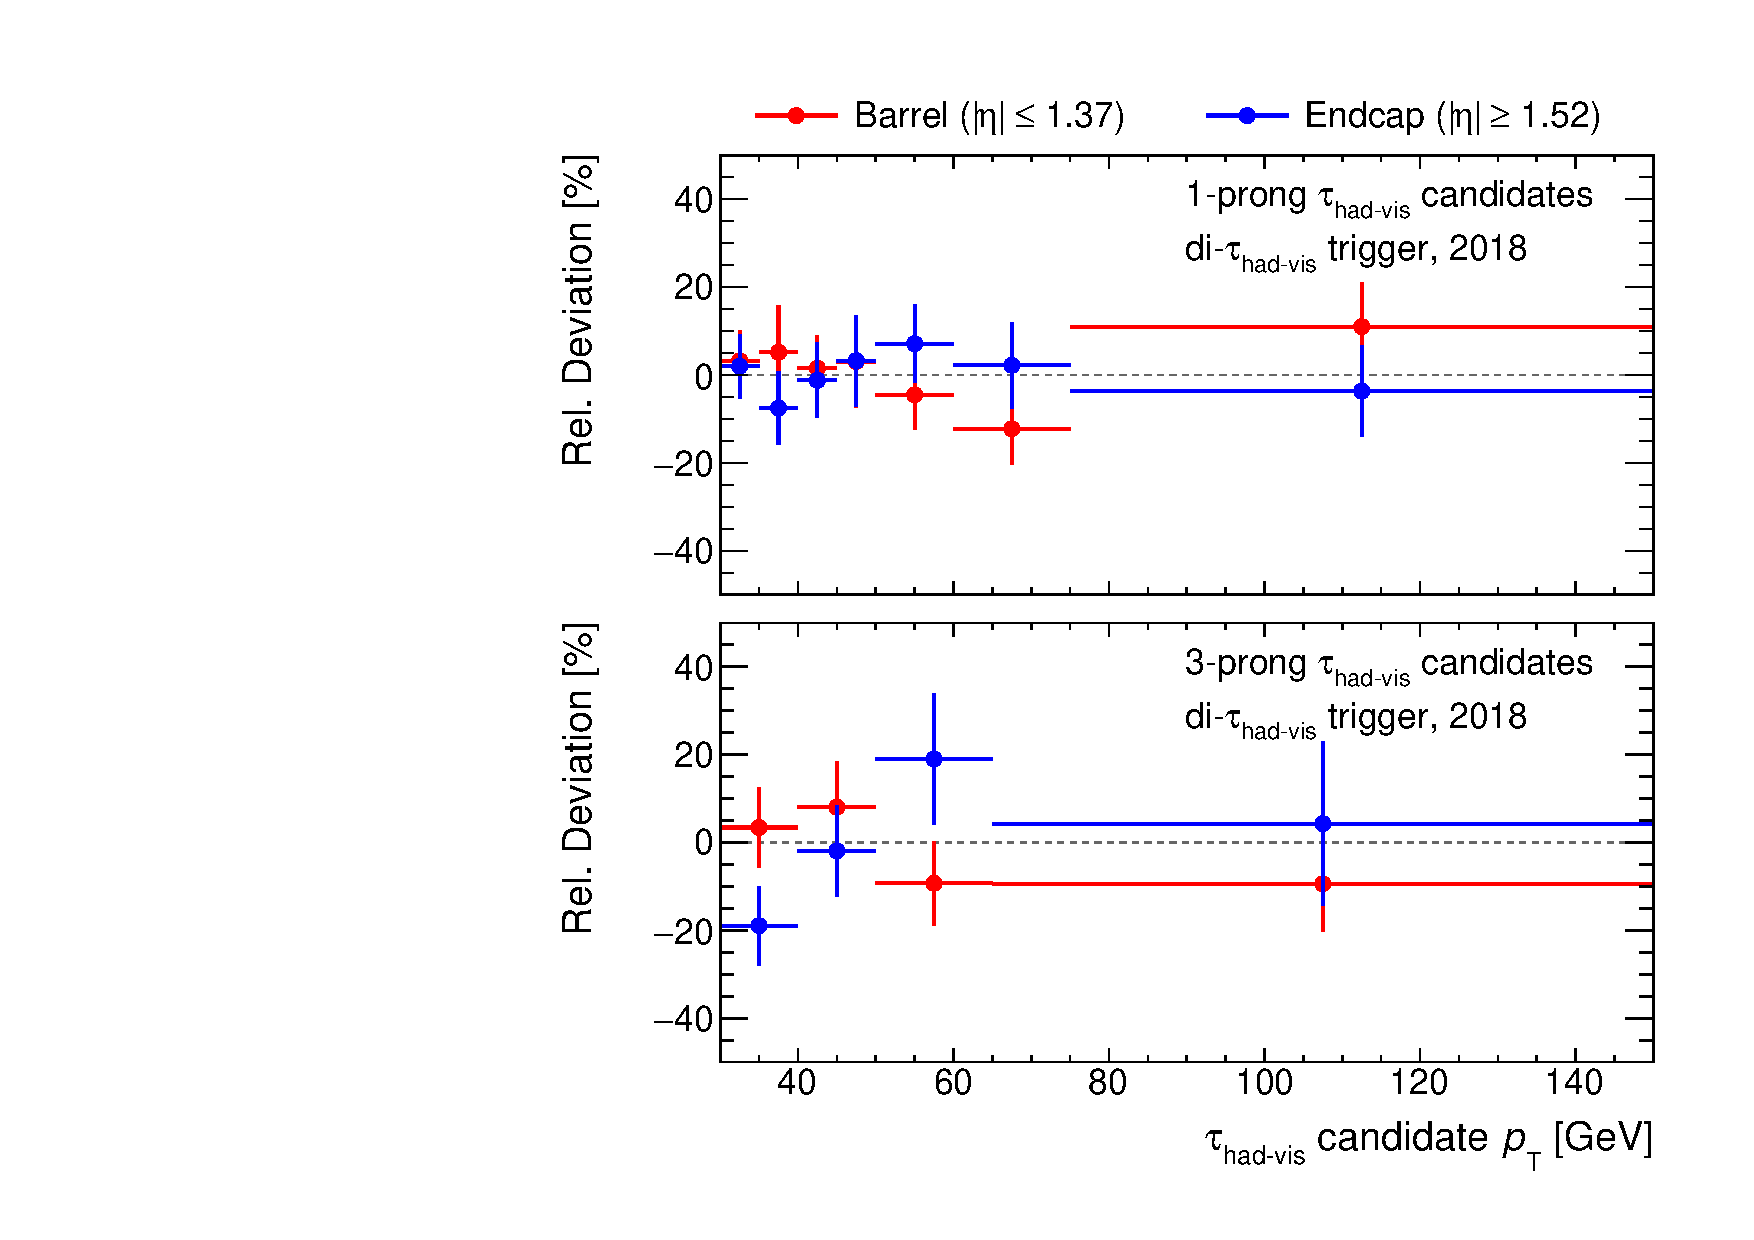
\includegraphics[width=\textwidth]{fakefactors/os_ss/fake_factors_osss_18}
    \subcaption{Comparison of OS and SS fake factors for events
      selected by di-\tauhadvis triggers. Only the 2018 data
      collection period is shown for illustration purposes.}
    \label{fig:fake_factor_OSSS_dtt}
  \end{subfigure}\hfill%
  \begin{subfigure}[t]{0.48\textwidth}
    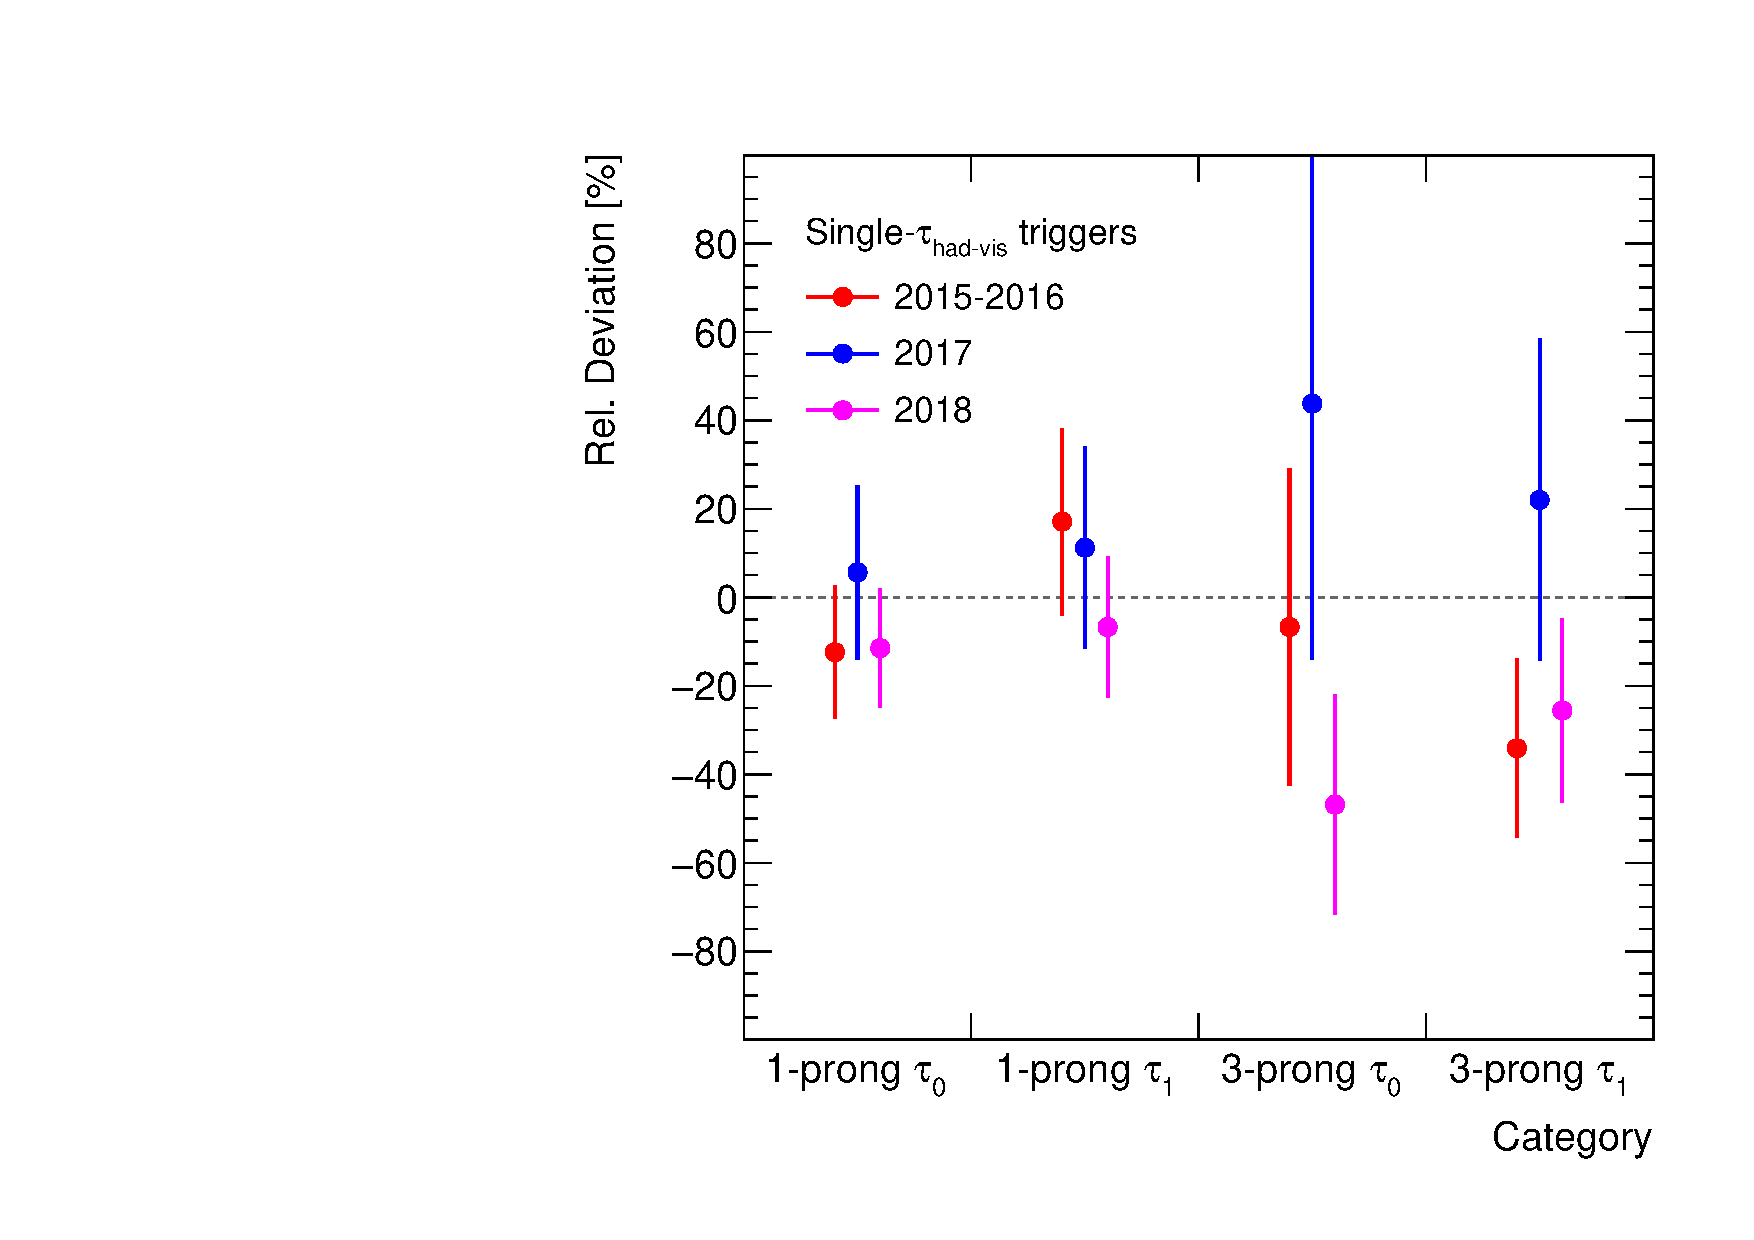
\includegraphics[width=\textwidth]{fakefactors/os_ss/fake_factors_osss_stt}
    \subcaption{Comparison of OS and SS fake factors for events
      selected by single-\tauhadvis triggers for all major data
      collection periods.}
    \label{fig:fake_factor_OSSS_stt}
  \end{subfigure}

  \caption{Relative deviation of fake factors measured in the 1
    $b$-tag OS multi-jet VR compared to the nominal set of fake
    factors measured in the 1 $b$-tag SS region (cf.\
    \Cref{fig:mjfakes_fake_factors,fig:mjfakes_stt_ffs}). The relative
    deviation is measured as $\FF_\text{OS} / \FF_\text{SS} - 1$ and
    is used to define a non-closure uncertainty that is propagated to
    the multi-jet background estimate when applying SS fake factors to
    events in OS regions. Statistical uncertainties from the finite
    number of observed data events and the non-multi-jet subtraction
    are shown.}
  \label{fig:fake_factor_OSSS}
\end{figure}


\subsubsection{Estimation of multi-jet backgrounds in the signal region}

The estimation of the multi-jet background in the \hadhad signal
region (2 $b$-tag OS ID) is obtained by applying fake factors from the
1 $b$-tag SS region to events in the 2 $b$-tag OS Anti-ID region after
subtraction of non-multi-jet processes. In addition, these fake
factors are multiplied by a 1 to 2 $b$-tag transfer factor to account
for possible differences between fake factors for 1 and 2 $b$-tag
regions (cf.\ \Cref{fig:fakefactor_regions}). The change in \btag
requirement is not expected to affect the measured fake factors, such
that the transfer factors mainly serve to provide a measurement-driven
estimate of the uncertainty on the extrapolation.

The transfer factor is determined by comparing fake factors measured
in the 2 $b$-tag SS region to ones extracted in the 1 $b$-tag SS
region. Due to the large multi-jet rejection of the 2 $b$-tag
requirement, the fake factors are measured inclusively in the trigger
category, \tauhadvis \pT and \tauhadvis $\eta$. The 1 to 2 $b$-tag
transfer factor is defined as the ratio
\begin{align*}
  \text{TF}_{1 \ra 2\,b\text{-tag}} = \frac{\FF_{\text{SS}}^{2\,b\text{-tag}}}{\FF_{\text{SS}}^{1\,b\text{-tag}}} \,\text{.}
\end{align*}

In~\Cref{fig:mjfakes_transfer_factor} the measured transfer factors
are shown. No statistically significant deviations between 1 and 2 $b$
-tag fake factors is observed. The statistical uncertainties on the
transfer factors are propagated to the multi-jet estimate in 2 $b$-tag
regions providing an extrapolation uncertainty.

%   - Large uncertainties indicate that we have little sensitivity to
%   the differences between 1- and 2-tag regions.

\begin{figure}[htbp]
  \centering

  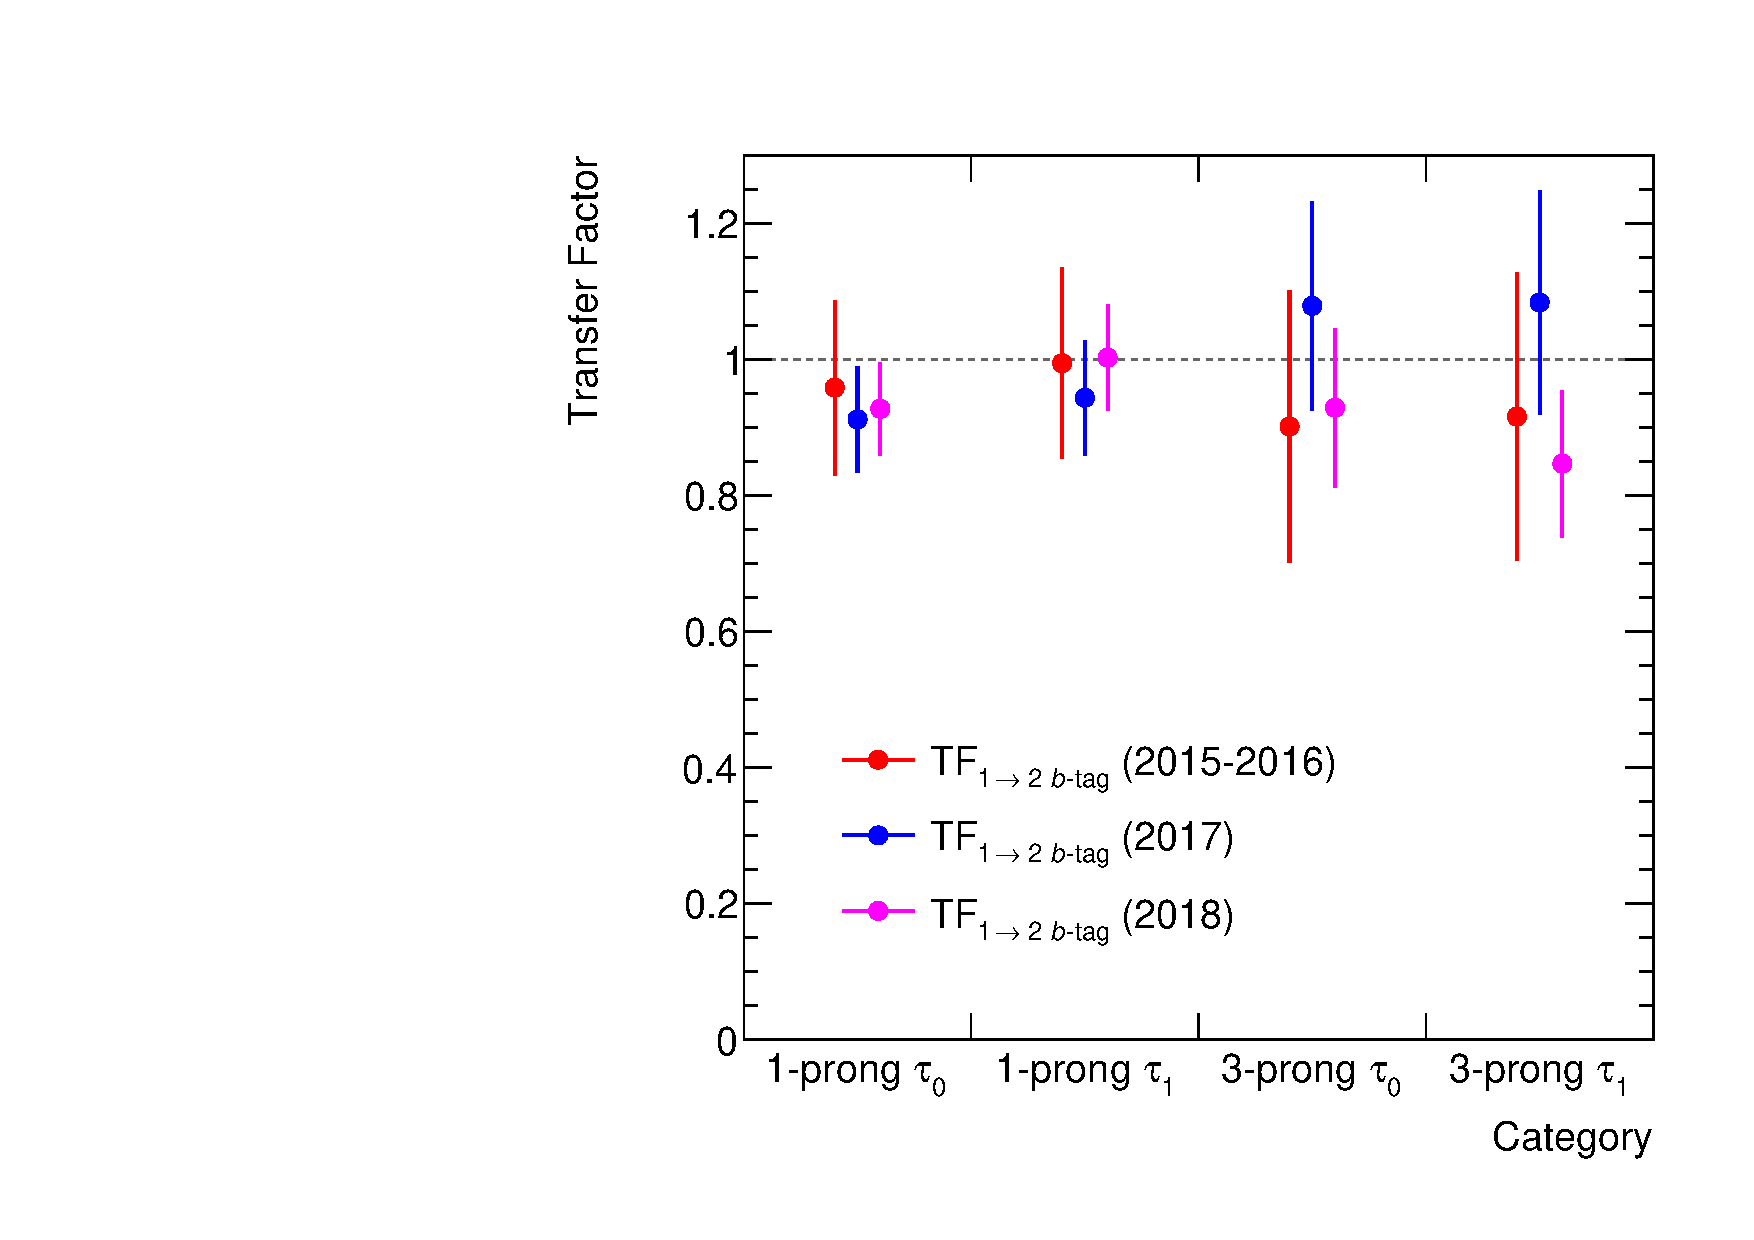
\includegraphics[width=0.495\textwidth]{fakefactors/transfer_factors}

  \caption{Transfer factors describing the ratio of fake factors
    measured in the 2 and 1 $b$-tag regions. The transfer factors are
    applied as multiplicative factors to 1 $b$-tag fake factors when
    they are applied in 2 $b$-tag regions. The statistical
    uncertainties are shown.}
  \label{fig:mjfakes_transfer_factor}
\end{figure}

A disadvantage of applying the fake factor method in the 2 $b$-tag
region is the low multi-jet purity of ca.\ \SI{50}{\percent} in the 2
$b$-tag OS Anti-ID region (cf.\
\Cref{tab:mjfakes_yields}). Resultingly, a large subtraction of
non-multi-jet processes has to be performed when applying fake factors
to obtain the multi-jet prediction in the signal region.  The size of
the subtraction in the 2 $b$-tag OS Anti-ID is illustrated
in~\Cref{fig:mjfakes_2tag_os_antiid}, showing that the dominant source
non-multi-jet events is \ttbarFakes. Due to the large relative size of
the subtracted non-multi-jet component, any uncertainties affecting
the subtracted components will have a large impact on the multi-jet
estimate in the ID region. This is the main limitation of the
multi-jet estimation method used in this analysis.

\todo[inline]{Refer to \Cref{sec:bkg_hadhad_ttbarfakes}.}

\begin{figure}[htbp]
  \centering

  \begin{subfigure}{0.49\textwidth}
    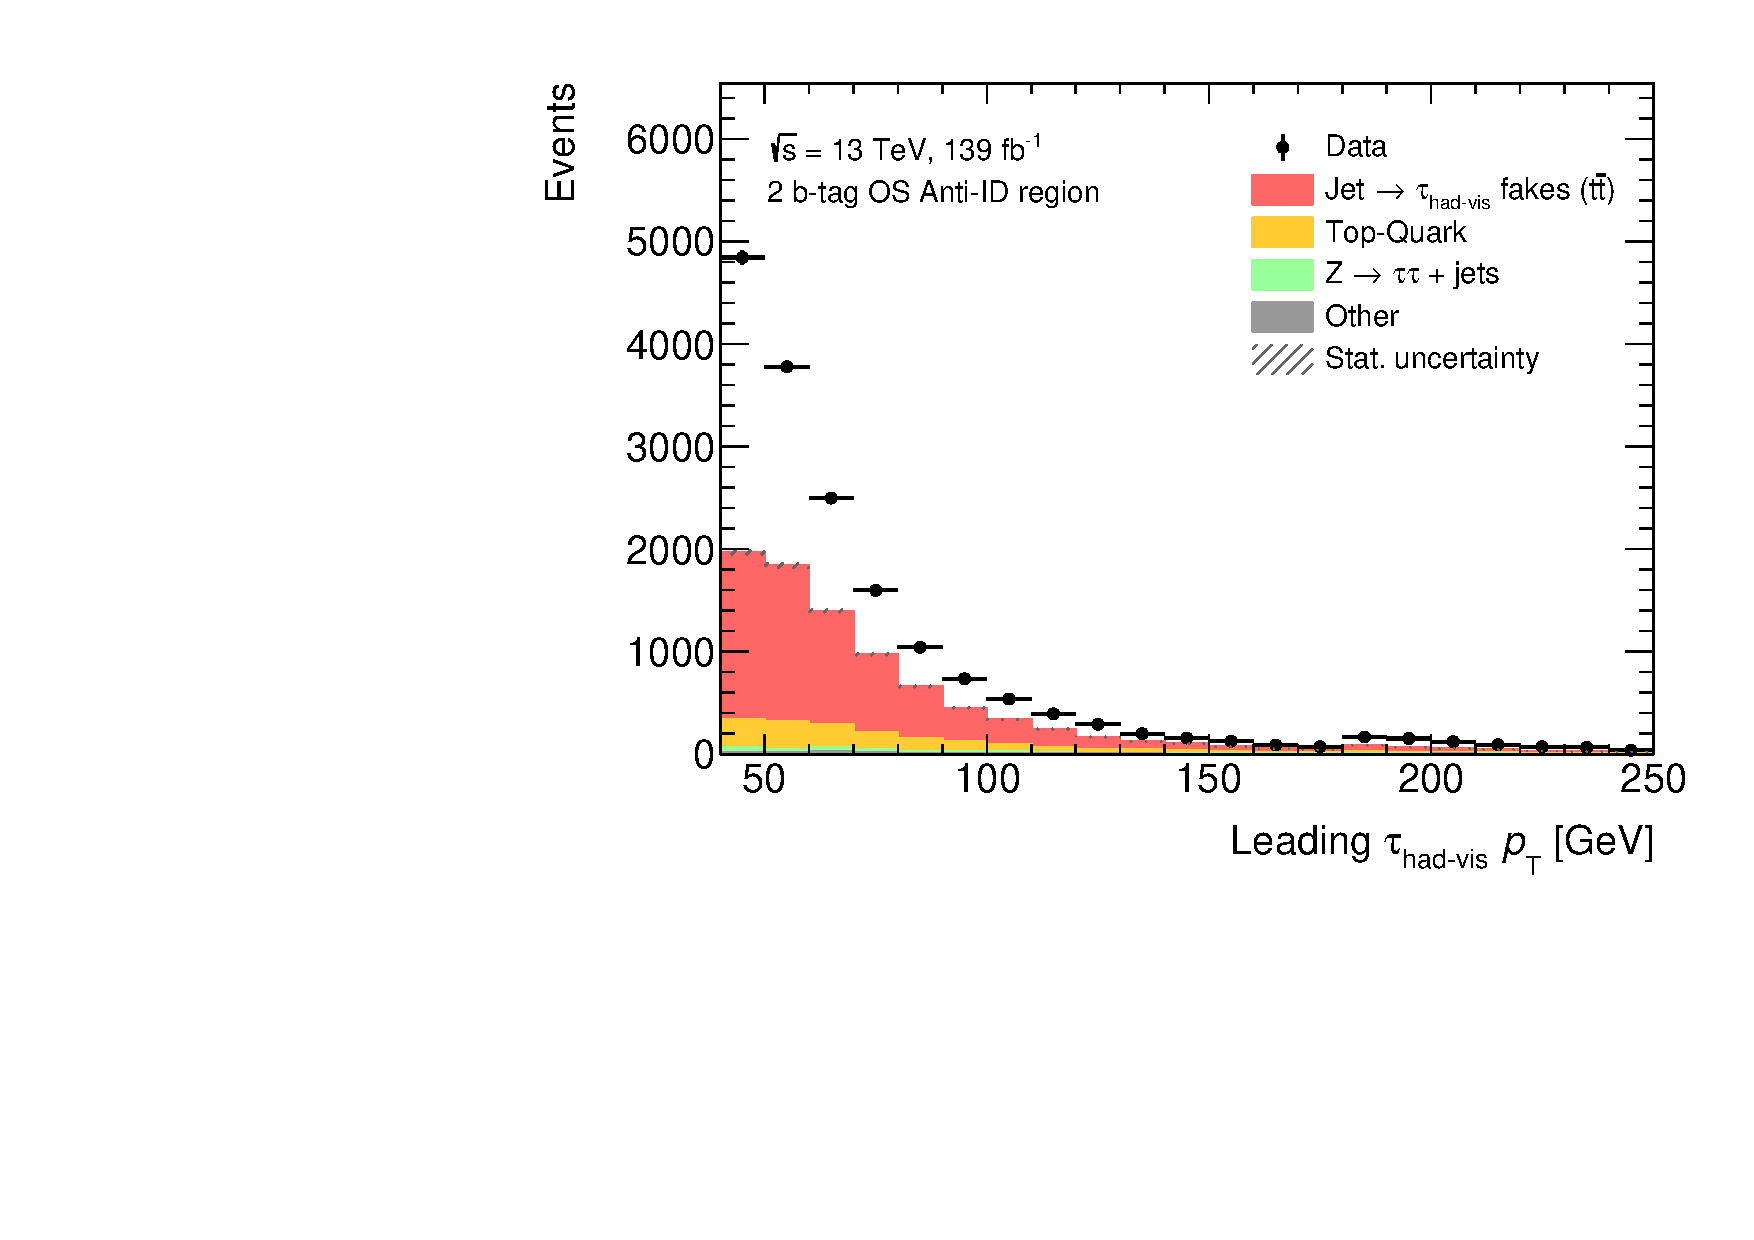
\includegraphics[width=\textwidth]{fakefactors/region_plots/tau0pt_2tag_os_antiid}
    \subcaption{}
  \end{subfigure}
  \begin{subfigure}{0.49\textwidth}
    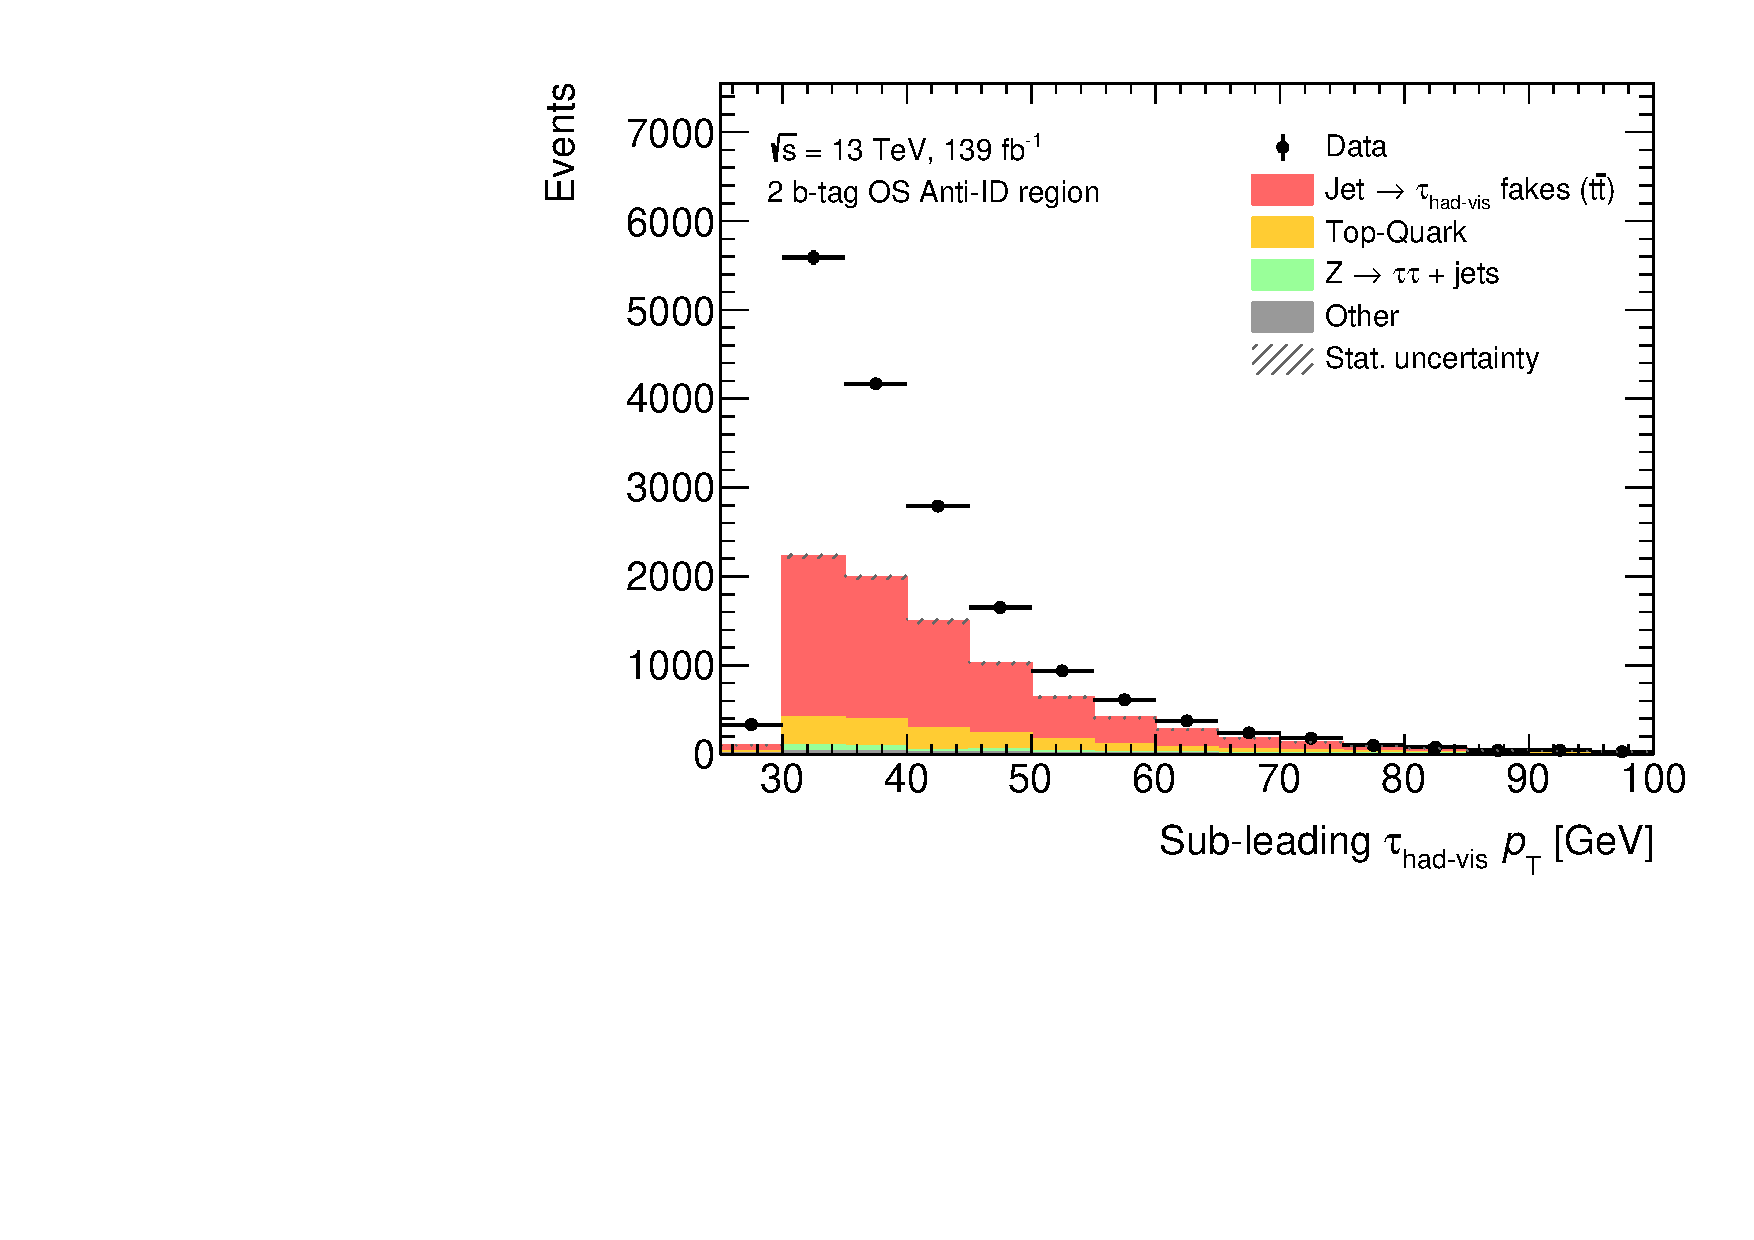
\includegraphics[width=\textwidth]{fakefactors/region_plots/tau1pt_2tag_os_antiid}
    \subcaption{}
  \end{subfigure}

  \caption{Histogram of the leading (a) and sub-leading (b) \tauhadvis
    candidate \pT in the 2 $b$-tag OS Anti-ID region. Non-multi-jet
    backgrounds are display as coloured histograms and include the
    statistical uncertainty of the prediction. The difference between
    the observed data and the non-multi-jet background prediction is
    attributed to the missing multi-jet estimate.}
  \label{fig:mjfakes_2tag_os_antiid}
\end{figure}


\subsubsection{Uncertainties}

% Statistical uncertainties
The statistical uncertainty of the multi-jet estimate due to the
finite number of observed events in the 2 $b$-tag OS Anti-ID region
and the simulation-based subtraction of non-multi-jet events. The
statistical uncertainty on the normalisation of the multi-jet
background in the \hadhad SR is \SI{1.9}{\percent}. % This uncertainty
% is included in the likelihood used for the statistical analysis by
% employing the Barlow-Beeston method~\cite{barlow1993,conway2011}.

The following systematic uncertainties are considered and propagated
to the multi-jet estimate in the \hadhad signal region:
\begin{itemize}
\item The statistical uncertainty of the fake factor measurement.

\item Non-closure uncertainty between fake factors estimated in the 1
  $b$-tag OS and SS regions.

\item Uncertainties on the extrapolation of fake factors measured in
  the 1 $b$-tag region to 2 $b$-tag regions.

\item Uncertainties on the subtraction of \ttbar, \ttbarFakes, and
  other non-multi-jet processes in the 2 $b$-tag OS Anti-ID region.
\end{itemize}

% Statistical uncertainty of FF (1.4 \%)
The effect of the statistical uncertainty on the multi-jet estimate in
the signal region is estimated by performing $\pm 1 \sigma$ variations
of individual bins of the fake factor measurement. The analysis is
insensitive to variations of individual fake factor bins and thus the
effect of all bins is combined into an overall normalisation
uncertainty on the multi-jet estimate. The normalisation uncertainty
on the multi-jet estimate originating from the statistical precision
of the fake factor measurement is \SI{1.4}{\percent}.

% Extrapolation uncertainty
An uncertainty on the extrapolation of fake factors measured in the 1
$b$-tag SS region to the 2 $b$-tag region is estimated by performing
$\pm 1 \sigma$ variations of the transfer factors. The four categories
of the transfer factor measurement are varied separately. As a
conservative estimate of the uncertainty, transfer factors of the
three major data collection periods are varied coherently within a
given category of the measurement.

% Transfer factor uncertainty (varying coherently all four categories)
% OS-SS uncertainty
%
% Subtraction uncertainty
%   ttbar (+16.8% -18.6%)
%   ttbar fakes
%   other (50% up and down)

% Dominant subtraction is ttbar, execpt for 1-tag OS ID where it is
% Ztautau.

% Signal contamination / other background contamination

% Yield table / plots of regions

\begin{table}[htbp]
  \centering

  % Nominal fake yield: 1354.7 +- 25.8 (1.9%)
% FF_OSSS__1down                                    +1.0 %
% FF_OSSS__1up                                      -1.0 %
% FF_OTHER_SUBTRACTION__1down                       +5.9 %
% FF_OTHER_SUBTRACTION__1up                         -5.9 %
% FF_TRUE_TTBAR_SUBTRACTION__1down                  +2.8 %
% FF_TRUE_TTBAR_SUBTRACTION__1up                    -2.5 %
% TF_STAT_1P_LEAD__1down                            -3.4 %
% TF_STAT_1P_LEAD__1up                              +3.4 %
% TF_STAT_1P_SUBL__1down                            -3.4 %
% TF_STAT_1P_SUBL__1up                              +3.4 %
% TF_STAT_3P_LEAD__1down                            -1.9 %
% TF_STAT_3P_LEAD__1up                              +1.9 %
% TF_STAT_3P_SUBL__1down                            -1.7 %
% TF_STAT_3P_SUBL__1up                              +1.7 %
% TTBAR_FAKESF_ANTITAU_DIFF__1down                  -2.1 %
% TTBAR_FAKESF_ANTITAU_DIFF__1up                    +2.1 %
% TTBAR_FAKESF_ANTITAU_OFFL_EIGEN0__1down           +0.1 %
% TTBAR_FAKESF_ANTITAU_OFFL_EIGEN0__1up             -0.1 %
% TTBAR_FAKESF_ANTITAU_TAU25EF_EIGEN0__1down        +2.1 %
% TTBAR_FAKESF_ANTITAU_TAU25EF_EIGEN0__1up          -2.2 %
% TTBAR_FAKESF_ANTITAU_TAU25RNN_EIGEN0__1down       +4.9 %
% TTBAR_FAKESF_ANTITAU_TAU25RNN_EIGEN0__1up         -5.1 %
% TTBAR_FAKESF_ANTITAU_TAU25_EIGEN0__1down          +4.2 %
% TTBAR_FAKESF_ANTITAU_TAU25_EIGEN0__1up            -4.3 %
\begin{tabular}{llr}
  \toprule
  \textbf{Source} &  \textbf{Nuisance parameter} & \textbf{Uncertainty}\\
  \midrule
  Statistical uncertainty & --$^\dagger$ & $\pm 1.9\,\%$ \\
  \midrule
  FF statistical uncertainty & \texttt{FF\_STAT\_HADHADSR} & $\pm 1.4\,\%$ \\
  \midrule
  Non-closure of OS / SS FFs & \texttt{FF\_OSSS} & $\pm 1.0\,\%$ \\
  \midrule
  1 to 2 $b$-tag extrapolation & \texttt{TF\_STAT\_1P\_LEAD} & $\pm 3.4\,\%$ \\
                               & \texttt{TF\_STAT\_1P\_SUBL} & $\pm 3.4\,\%$ \\
                               & \texttt{TF\_STAT\_3P\_LEAD} & $\pm 1.9\,\%$ \\
                               & \texttt{TF\_STAT\_3P\_SUBL} & $\pm 1.7\,\%$ \\
  \midrule
  \ttbar subtraction & \texttt{FF\_TRUE\_TTBAR\_SUBTRACTION} & $\pm 2.8\,\%$ \\
  \midrule
  \ttbarFakes subtraction & \texttt{TTBAR\_FAKESF\_ANTITAU\_DIFF} & $\pm 2.1\,\%$ \\
                                 & \texttt{TTBAR\_FAKESF\_ANTITAU\_OFFL\_EIGEN0} & $\pm 0.1\,\%$ \\
                                 & \texttt{TTBAR\_FAKESF\_ANTITAU\_TAU25\_EIGEN0} & $\pm 4.3\,\%$ \\
                                 & \texttt{TTBAR\_FAKESF\_ANTITAU\_TAU25EF\_EIGEN0} & $\pm 2.2\,\%$ \\
                                 & \texttt{TTBAR\_FAKESF\_ANTITAU\_TAU25RNN\_EIGEN0} & $\pm 5.1\,\%$ \\
  \midrule
  Other subtraction & \texttt{FF\_OTHER\_SUBTRACTION} & $\pm 5.9\,\%$ \\
  \bottomrule
\end{tabular}

%%% Local Variables:
%%% mode: latex
%%% TeX-master: "../phd_thesis"
%%% End:


  \caption{Impact of uncertainties on the normalisation of the
    multi-jet estimate in the \hadhad signal region. Shape effects of
    variations are propagated to the multi-jet estimate with the
    exception of \texttt{FF\_STAT\_HADHADSR}. The treatment of
    statistical uncertainties ($\dagger$) in the context of
    likelihood-based tests will be discussed in~REFERENCE.}
  \label{tab:multi_jet_uncertainties}
\end{table}

Systematic uncertainties are assigned to cover possible difference
betwen OS and SS fake factors, varying the subtraction in the OS
Anti-ID region. Moreover, the fake factors are independently varied by
their statistical uncertainty.

\todo[inline]{Could we use nOS to enhance statistics? Maybe flip the FF method
  so that we use events in SS ID to build the template instead of OS Anti-ID.}

\todo[inline]{Can we make the STT FF depend on the trigger-match instead of
  the leading / subleading binning?}

%%% Local Variables:
%%% mode: latex
%%% TeX-master: "../../phd_thesis"
%%% End:
